\documentclass[journal]{IEEEtran}

% *** GRAPHICS RELATED PACKAGES ***
%
\ifCLASSINFOpdf
  % \usepackage[pdftex]{graphicx}
  % declare the path(s) where your graphic files are
  % \graphicspath{{../pdf/}{../jpeg/}}
  % and their extensions so you won't have to specify these with
  % every instance of \includegraphics
  % \DeclareGraphicsExtensions{.pdf,.jpeg,.png}
\else
  % or other class option (dvipsone, dvipdf, if not using dvips). graphicx
  % will default to the driver specified in the system graphics.cfg if no
  % driver is specified.
  % \usepackage[dvips]{graphicx}
  % declare the path(s) where your graphic files are
  % \graphicspath{{../eps/}}
  % and their extensions so you won't have to specify these with
  % every instance of \includegraphics
  % \DeclareGraphicsExtensions{.eps}
\fi
% graphicx was written by David Carlisle and Sebastian Rahtz. It is
% required if you want graphics, photos, etc. graphicx.sty is already
% installed on most LaTeX systems. The latest version and documentation
% can be obtained at: 
% http://www.ctan.org/tex-archive/macros/latex/required/graphics/
% Another good source of documentation is "Using Imported Graphics in
% LaTeX2e" by Keith Reckdahl which can be found at:
% http://www.ctan.org/tex-archive/info/epslatex/
%
% latex, and pdflatex in dvi mode, support graphics in encapsulated
% postscript (.eps) format. pdflatex in pdf mode supports graphics
% in .pdf, .jpeg, .png and .mps (metapost) formats. Users should ensure
% that all non-photo figures use a vector format (.eps, .pdf, .mps) and
% not a bitmapped formats (.jpeg, .png). IEEE frowns on bitmapped formats
% which can result in "jaggedy"/blurry rendering of lines and letters as
% well as large increases in file sizes.
%
% You can find documentation about the pdfTeX application at:
% http://www.tug.org/applications/pdfte

% correct bad hyphenation here
\hyphenation{op-tical net-works semi-conduc-tor}

\usepackage{graphicx}
\usepackage{amsmath}
\usepackage{amssymb}
\usepackage{color}
\usepackage{epsfig}
\usepackage{tabularx}
\usepackage{ctable}
\usepackage{multirow}
\usepackage{subfigure}
\usepackage{mathrsfs}
\usepackage{mathtools}
\usepackage{hyperref}
\usepackage{algorithm}
\usepackage{algpseudocode}
\usepackage{booktabs}
\usepackage{sci}
% gray scaled table
%\newcommand\gray{gray}
%
%\newcommand\ColCell[1]{%
  %\pgfmathparse{#1<.6?1:0}%
    %\ifnum\pgfmathresult=0\relax\color{white}\fi
  %\pgfmathparse{1-#1}%
  %\expandafter\cellcolor\expandafter[%
    %\expandafter\gray\expandafter]\expandafter{\pgfmathresult}#1}
%
%\newcolumntype{E}{>{\collectcell\ColCell}c<{\endcollectcell}}


% format argmin
%\DeclareMathOperator*{\argmin}{arg\,min}

% algorithm title
%\makeatletter
%\def\BState{\State\hskip-\ALG@thistlm}
%\makeatother

\newcommand{\songfan}[1]{\textcolor{blue}{#1}}




\begin{document}
%
% paper title
% can use linebreaks \\ within to get better formatting as desired
% Do not put math or special symbols in the title.
\title{Person-Independent Facial Expression  \\ Recognition Using Low-Rank Expression \\ and Sparse Expression Residual}
%
%
% author names and IEEE memberships
% note positions of commas and nonbreaking spaces ( ~ ) LaTeX will not break
% a structure at a ~ so this keeps an author's name from being broken across
% two lines.
% use \thanks{} to gain access to the first footnote area
% a separate \thanks must be used for each paragraph as LaTeX2e's \thanks
% was not built to handle multiple paragraphs
%

\author{Songfan~Yang,~\IEEEmembership{Member,~IEEE,}
				Le~An,~\IEEEmembership{Member,~IEEE,}
				Yinjie~Lei,~\IEEEmembership{Member,~IEEE,}
        and~Bir~Bhanu,~\IEEEmembership{Fellow,~IEEE}% <-this % stops a space
\thanks{S.~Yang and Y.~Lei are with the College of Electronics and Information Engineering at Sichuan University, Chengdu, China 610064. E-mail: \{syang,~yinjie\}@scu.edu.cn}
\thanks{L.~An is the Department of Electrical and Computer Engineering, University of California, Riverside, CA 92521 USA. E-mail: lan004@ucr.edu}
\thanks{B.~Bhanu is with the Center for Research in Intelligent Systems, University of California, Riverside, CA 92521 USA. E-mail: bhanu@cris.ucr.edu}
}


% The paper headers
\markboth{IEEE Transaction on Multimedia,~Vol.~, No.~, }%
{Shell \MakeLowercase{\textit{et al.}}: Bare Demo of
IEEEtran.cls for Computer Society Journals}
% make the title area
\maketitle

% As a general rule, do not put math, special symbols or citations
% in the abstract or keywords.
\begin{abstract}
Person-independent expression recognition aims to recognize facial expressions of an \textit{unseen} subject. This remains a challenging problem due to that the facial muscle motion for a typical facial expression, which should be similar irrespective of the subject's identity, is difficult to quantify and generalize across population. Therefore, trained classifiers can easily over-fitted to person-specific facial appearances rather than to person-independent muscle motion from expressions. This problem becomes even more challenging when the rigid head motion and non-rigid facial muscle motion are observed in uncontrolled videos. To tackle these challenges, we model an facial expression video as a combination of two parts: 1) a set of low-rank components that represent person-independent expression prototypes, termed as Low-Rank Expression (LRE), and 2) a set of sparse appearance residuals that capture the muscle motion of individual frames in video, namely Sparse Expression Residual (SER). To avoid over-fitting, we explicitly model the person-independent transformation of individual frames with respect to a canonical reference space, in terms of an objective function to be minimized. We show that this objective function can be simplified and solved by an efficient sparse low-rank recovery algorithm. A comparative study between the state-of-the-art models and the proposed LRE representation shows the merits of our approach in representing expressions in a person-independent manner. We also demonstrate that the SER can also be utilized to further improve the recognition performance, when both spatial and temporal texture features are extracted out of SER. Extensive qualitative and quantitative results demonstrate the superiority of our approach as compared to most recent methods.

\end{abstract}

% Note that keywords are not normally used for peerreview papers.
\begin{IEEEkeywords}
Facial expression recognition, person-independent, low-rank expression, sparse expression residual
\end{IEEEkeywords}






% For peer review papers, you can put extra information on the cover
% page as needed:
% \ifCLASSOPTIONpeerreview
% \begin{center} \bfseries EDICS Category: 3-BBND \end{center}
% \fi
%
% For peerreview papers, this IEEEtran command inserts a page break and
% creates the second title. It will be ignored for other modes.
\IEEEpeerreviewmaketitle



\section{Introduction}

\IEEEPARstart{A}{ffective} computing has been attracting an increasing amount of attentions in both psychology and computer science studies~\cite{Picard03}. As a primary channel to convey emotion, facial expression contains rich information and has been extensively studied~\cite{Pantic_PAMI00,Torre11}. Although a rich body of research on facial expression recognition in controlled environments was conducted~\cite{Torre11}, a recent expression analysis challenge~\cite{FERA11} indicates that person-independent expression recognition in video remains a difficult problem in uncontrolled settings, due to the following reasons:

\begin{figure}[t]
	\centering
		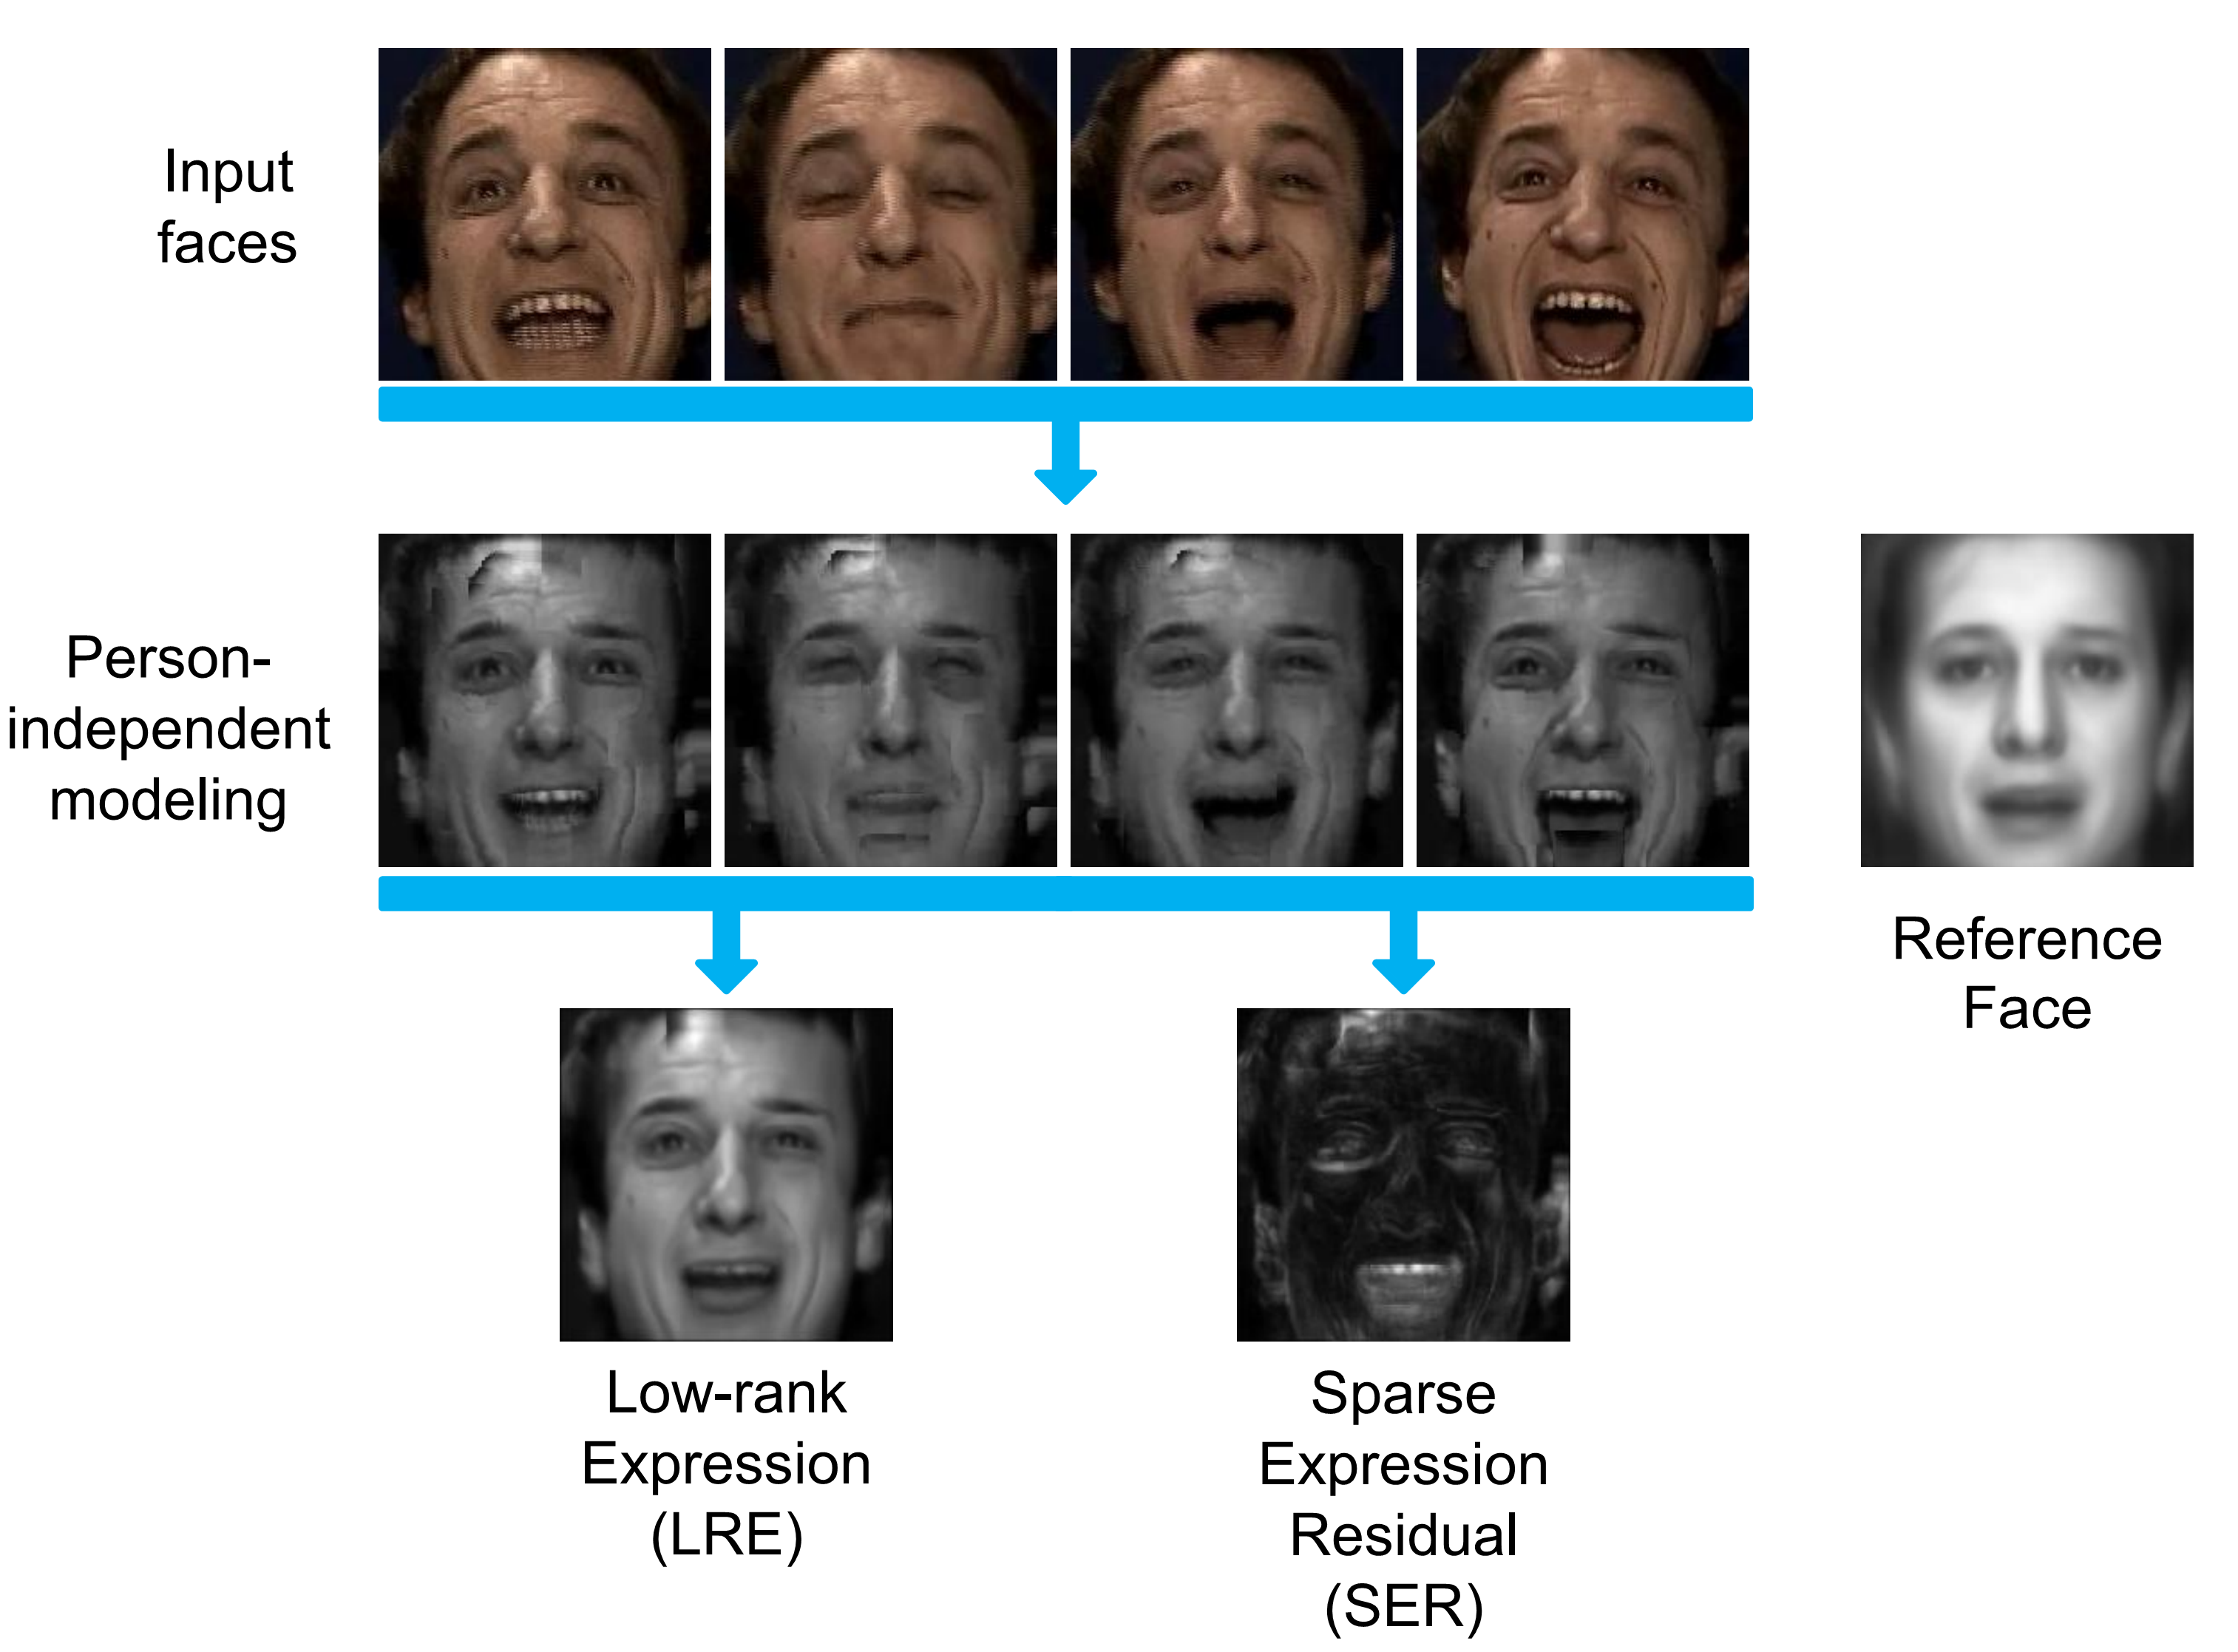
\includegraphics[width=.95\columnwidth]{pics/splash.png}
	\caption{The overview of our approach. We observe that: 1) a facial expression sequence possess an inherent \textit{global} model (\textit{e.g.}, lip corner expansion for \textit{Happiness} in this case); and 2) each frame has its own \textit{local} properties (\textit{e.g.}, various muscle motion intensities), which describe the facial dynamics. Due to the face anatomy constraints~\cite{Ekman78}, the muscle motion that characterize the local deformation is sparsely distributed. Inspired by these observations, we model each frame as: 1) a Low-Rank Expression (LRE) that represents the global expression appearance estimated from the entire sequence; and 2) an additive Sparse Expression Residual (SER) that represents the deviations from the low-rank structure. Moreover, the person-independent factor is modeled as a transformation with respect to a canonical space (reference face), avoiding over-fitting for classification. Both LRE and SER provide viable manners to extract meaningful facial expression dynamics, yielding superior recognition performances. To appreciate the information captured by the LRE and SER representations, the bottom row shows the mean representation of the decomposed sequence. The mean LRE retains the global appearance and the mean SER captures the local motion around mouth and eye regions.}
	\label{fig:splash}
\end{figure}

\begin{enumerate}

\item \textbf{Compound motion.} In real-world scenarios, the facial expression appearance in video consists of rigid head motion and non-rigid muscle motion. The rigid head motion includes both in-plane and out-of-plane rotations. Aligning 2D faces by rectifying the out-of-plane rotation is considerably more difficult than dealing with in-plane rotation due to the complexity in 3D human face. Most approaches in the literature only recover the in-plane rotation by computing an affine transformation based on facial feature correspondences~\cite{Bartlett_FG11,Valstar_FERA11}. Furthermore, segmenting the non-rigid muscle motion from the rigid head motion, which reveals the true facial expression, is an inherently challenging problem from 2D images.

\item \textbf{Person-specific effect.} Psychological study shows that there are six basic prototype expressions that have similar properties across various cultures, namely, \textit{Happiness}, \textit{Sadness}, \textit{Surprise}, \textit{Fear}, \textit{Anger}, and \textit{Disgust}~\cite{Fridlund_87}.  Many vision-based expression analyses rely on these basic prototypes~\cite{Pantic_PAMI00}.  An ``ideal'' expression recognition system is expected to eliminate cultural-independent and even person-independent information. However, typical facial expression recognition systems use generic appearance or geometry-based features to characterize an expression, without taking into account the person-specific property~\cite{Bartlett_FG11,Valstar_SMCB12}. Thus, person-specific information is retained and the classifier may fail to recognize person-independent expressions. This results in an over-fitted classification model that ultimately degrades the recognition accuracy on unseen testing subjects. There has been some pioneer work~\cite{Yang_SMCB12,Dahmane_TMM14} that attempts to alleviate the person-specific effect, and the improved results have verified that person-independent modeling is a key issue in obtaining robust expression recognition systems.

\end{enumerate}

In this paper, the problem we intend to solve is as follows: given a video sequence of a facial expression after temporal segmentation, the goal is to classify each segment of this video as one of the six categorical expression, \textit{e.g.}, \textit{Happiness} or \textit{Anger}. 

Previous approaches for this task can be categorized into three strategies for video-based expression recognition. In the first category, a wide range of methods~\cite{Bartlett_FG11,Valstar_SMCB12} process each frame individually and a majority voting rule is applied to determine the expression type for the entire sequence. In the second category, temporal features are used to capture the muscle dynamics of facial expressions~\cite{Zhao_PAMI07,Huang11}. These approaches typically require accurate facial alignment in order to generate meaningful dynamic features. In the third category, an entire video sequence is summarized into an image-based representation that captures the expression appearance~\cite{Yang_SMCB12,Dahmane_TMM14}. These approaches completely abandon the dynamic information, and cannot model the temporal characteristic of facial expressions. In essence, the aforementioned strategies summarize the video-based expression data at different resolution. 

In this work, we depart from all the previous strategies and analyze the facial expression at a finer resolution. We observe that, on one hand, expressions in individual frames from one video sequence are correlated and possess similar \textit{global} characteristics (\textit{e.g.}, lip corner expansion for \textit{Happiness}); on the other hand, each sample has its own \textit{local} properties (\textit{e.g.}, various muscle motion intensities for different expression stages such as \textit{onset}, \textit{apex}, or \textit{offset}), which could be used to describe facial dynamics. Due to the face anatomy constraints~\cite{Ekman78}, the muscle motion that characterizes the local deformation is sparsely distributed. 

Inspired by these observations, we model each frame as 1) a Low-Rank Expression (LRE) that represents the global expression appearance estimated from the entire sequence; and 2) an additive sparse expression residual (SER) that represents the deviations from the low-rank structure. As shown in Fig.~\ref{fig:splash}, both static and dynamic features are extracted from LRE and SER representations for expression recognition. In addition, we explicitly model the person-independent facial expression appearance transformation in a low-rank recovery framework. The person-independent factor is modeled as a non-linear transformation function, which can be approximated by matching a target face to a canonical reference face. Concretely, we approximate this non-linearity by the correspondence of two SIFT feature descriptors, namely SIFT-flow~\cite{Liu_PAMI11}. We then show that the person-independent transformation is independent of the low-rank recovery procedure, leading to an efficient algorithm in the pursuit of the sparse low-rank facial expression appearances. 

In what follows, Section~\ref{sec:related} reviews the related work in the literature and highlights our contributions. Subsequently, Section~\ref{sec:decompose} details the modeling of expression images as LRE and SER representations, and contrast them with previous approaches in theory and practice. Section~\ref{sec:exp} demonstrates the effectiveness of LRE+SER modeling via extensive experimental results. Finally, Section~\ref{sec:conclude} concludes this paper.

%In particular, in Section~\ref{sec:eai}, we discuss the relationship of LER with the Emotion Avatar Images (EAI)~\cite{Yang_SMCB12} in terms of both theory and results.


\section{Related Work and Our Contributions\label{sec:related}}

We first review the related works in the literature for both facial expression recognition and sparse representation, and highlight our contributions thereafter. 

\subsection{Facial Expression Recognition}

Automatic facial expression analysis has been studied extensively. Earlier work mainly focuses on recognizing expressions from \textit{static} images, where both facial geometry and textures are used for this task~\cite{Pantic_PAMI00,Essa_PAMI97,Donato_PAMI99}. Recent work in expression analysis deals with videos~\cite{Bartlett_FG11,Kaliouby_SMC04,Valstar_FERA11}. These systems treat each frame individually and attempt to recognize facial expression or Action Units (AUs)~\cite{Ekman78}. For feature representations in facial expression analysis, the texture features can be described using Haar-like features~\cite{Whitehill_FG06}, Gabor filters~\cite{Lyons_PAMI99,Bartlett_FG11}, Local Binary Patterns (LBP)~\cite{Shan_IVC09,Jiang_FG11}, Edge Orientation Histogram~\cite{Levi_CVPR04}, Histogram of Oriented Gradients (HOG)~\cite{Dalal_CVPR05,Dhall_FERA11,Dahmane_FERA11}, and Local Phase Quantization (LPQ)~\cite{LPQ}, etc.

As pointed out in~\cite{Ekman2005} and~\cite{Ambadar05}, facial muscle \textit{dynamics} play an important role in spontaneous expressions. The pioneer work by Yacoob and Davis~\cite{Yacoob_PAMI96} describes the facial dynamics using optical flow. It is assumed that subjects are with controlled frontal head pose, and thus, a simple thresholding procedure can rule out small motion cause by noise or tracking errors. This assumption immediately raises concern since optical flow highly relies on accurate face tracking and alignment. Moreover, this work ignores the facial texture information, which is important in characterizing facial dynamics. For example, Zhao and Pietik\"ainen~\cite{Zhao_PAMI07} extend LBP to the temporal space, namely three orthogonal planes (LBP-TOP), by taking into account the co-occurrence of the patterns. It combines appearance and motion together and achieves outstanding performance for facial expression recognition under controlled settings, \textit{e.g.}, the Cohn-Kanade database~\cite{CKplus}. Similarly, various texture descriptors, \textit{e.g.}, LPQ-TOP~\cite{LPQ-TOP}, can be extended to spatial-temporal settings, yielding a superior performance. The muscle dynamics can also be characterized by the motion of facial landmarks (\textit{e.g.}, eyebrow corner, mouth corner, etc.). Valstar and Pantic~\cite{Valstar_SMCB12} track a set of landmarks over time and infer facial expressions based on the dynamics of landmark. 

Facial dynamics are easier to capture in controlled settings~\cite{CKplus}, where subjects are constraint to have limited head motion and exaggerated facial muscle motion. However, in a more realistic and uncontrolled scenario (\textit{e.g.}, FERA dataset~\cite{Valstar_FERA11}), extracting facial dynamics highly relies on accurate facial landmark tracking and face alignment. The facial expression in real world consists of the ``compound motion'' from the rigid head motion and deformable facial muscle motion. Ideally, the head motion should be corrected to fully characterize the non-rigid muscle motion, which is directly related to the expressions. It is shown in~\cite{Valstar12,Yang_SMCB12} that without a reliable alignment, using the dynamic feature is even inferior than simply using static features. Therefore, in this work, we establish a framework that aligns expression images under compound motion from region-based correspondences (in contrast to point-based correspondences), which helps to extract much more effective dynamic features. 


\subsection{Sparse Representation}

Recently, sparse modeling has witnessed its success in diverse applications such as image restoration~\cite{Yang_CVPR08}, face recognition~\cite{Wright_PAMI09}, and human action recognition~\cite{Qiu_ICCV11}. In particular, sparse representation combined with low-rank modeling can be used to extract robust features directly from an image in a matrix form, such as the transform invariant low-rank textures~\cite{Zhang_IJCV12}, group alignment by sparse and low-rank decomposition~\cite{Peng_PAMI12}. In the facial expression related domain, the method proposed in~\cite{Lin12} jointly recovers a dictionary and a set of sparse coefficients to efficiently synthesize 3-D facial expressions. In~\cite{Tariq12} the mid-level features are learned by sparse coding technique for multi-view expression recognition. It uses sparse codes of local descriptors (such as SIFT) to build features for expression recognition. Different from these approaches, in this work we focus on recovering 2D representations that are of low-rank property for a better performance in facial expression recognition. 

\subsection{Our Contributions}
The contributions of this work are the follows:
\begin{enumerate}
\item We observe that each frame of a prototype expression sequence is correlated and composed of a global and a local component. We then propose to model the generic person-independent facial expressions video in a sparse low-rank recovery framework. The sequence is decomposed into two components, termed Low-Rank Expression (LRE) and Sparse Expression Residual (SER), which jointly help to extract more effective dynamic facial features, leading to a superior recognition performance. 
\item We show that a special case of person-independent transformation, via SIFT-flow, results in a low-rank expression model, which visually resembles the Emotion Avatar Image (EAI) representations~\cite{Yang_SMCB12}. As shown by the experimental results, this transformation can well handle unseen data during testing.
%\item We demonstrate that the non-rigid muscle motion captured by the sparse residual component, SER, is an effective representation to extract dynamics from and can further improve the recognition performance. Both quantitative and qualitative evaluations are carried out to justify the improvement. 
\end{enumerate}

\section{Person-independent Expression Modeling\label{sec:decompose}}

\subsection{The Generalized Model} 
We assume that a video is temporally segmented such that each segment can be described by one prototype expression or an AU. We then seek to decompose each frame of the sequence into two representations, LRE and SER, to capture the global appearance of the segment and non-rigid muscle motion for each frame, respectively. Formally, given a sequence of video segment, we denote $\I_1, \ldots, \I_n$ as $n$ image observations of the sequence. Then each frame can be decomposed as

\begin{equation}
\I_i = \I^{0}_i + \R_i,\quad i = 1\cdots n,
\end{equation}
where sparse residual is modeled by the additive term $\R_i$. $\I^{0}_i$ is the difference between $\I_i$ and $\R_i$. Furthermore, we denote $\v\in\mathbb{R}^{m}$ to be the vectorized observation of $\I_i$ and $\e_i$ to be the vectorized version of $\R_i$. Stacking multiple such vectors results in an observation matrix

\begin{equation}
\D = [\v_1,  \cdots, \v_n] = \A + \E,
\end{equation}
where $D\in\mathbb{R}^{m\times n}$, and $\A = [\v^{0}_{1}, \cdots, v^{0}_{n}]$ is a low-rank matrix that models the dominant structure of the facial expression sequence. $\E = [\e_{1}, \cdots, \e_{n}]$ is a sparse matrix with large non-zero elements representing the motion of the sequence. Thus, the problem that we try to solve is

\begin{equation} \label{eq:org}
\min_{\A,\E} rank(\A)+\gamma \|\E\|_0,  \quad \text{s.t.} \quad \D = \A + \E, 
\end{equation}
where $\|\cdot\|_0$ is the $\ell_0$ norm counting the number of non-zero entries in the error term $\E$. $\gamma$ is a scaling parameter which controls a weight preference of the rank of $\A$ and sparsity of $\E$. Although (\ref{eq:org}) is an intuitive formulation, it is a non-convex and NP-hard problem which is difficult to solve. As suggested by many works in sparse low-rank recovery~\cite{Candes11,Lin09,Peng_CVPR10}, (\ref{eq:org}) can be relaxed by its convex surrogate as

\begin{equation}
\min_{\A,\E} \|\A\|_*+\gamma \|\E\|_1,  \quad \text{s.t.} \quad \D = \A + \E, 
\end{equation}
where $\|\cdot\|_*$ is the nuclear norm that computes the sum of all singular values of $\A$, and $\|\E\|_1=\sum_{ij}|\E_{ij}|$. This new objective is convex and can be solve by an efficient first-order accelerated proximal gradient algorithm~\cite{Lin09,Beck09}. 


\subsection{Reference-based Person-Independent Transformation} 

Since a face in each frame $\I_i$ contains pose and identity variations, we intend to carry out the expression recognition task in a canonical space. Specifically, we model the person-independent factor by mapping each face to a reference face model, $\I_r$. This strategy has been demonstrated effective in expression recognition, particularly in predicting expressions for unseen subjects~\cite{Yang_SMCB12,Dahmane_TMM14}. We model the mapping by a transformation function applied to each frame of the entire sequence. Thus, the objective is written as

\begin{equation}
\min_{\A,\E} \|\A\|_*+\gamma \|\E\|_1  \quad \text{s.t.} \quad \phi (\D) = \A + \E. 
\end{equation}

Here, $\phi (\D)$ is defined as a generic function that transforms each face $\I_i$ in $\D$ to the canonical space. One instantiation of the non-linear mapping, which we employ in this work, is SIFT-flow that performs structural matching~\cite{Liu_PAMI11}. 

SIFT-flow was originally designed to align an image to its plausible nearest neighbor which can have large variations. It robustly matches dense structural SIFT features between two images, while maintaining spatial discontinuities. The SIFT~\cite{Lowe_ICCV99} features are first extracted in a pixel-wise fashion. For every pixel in an image, the neighborhood (\textit{e.g.}, $16\times16$) is divided into a $4\times4$ cell array. The orientation of each cell is quantized into 8 bins, generating a $4\times4\times8=128$-dimensional vector as the SIFT representation for a pixel. Subsequently, a dense correspondence is established to match the two SIFT images. Similar to optical flow, the objective energy function is designed as
\begin{align}
	\label{data_term}
	E(\w)=&\sum_\p \min (\left\|\s_1 (\p)-\s_2 (\p+\w(\p))\right\|_1 ,t)+
\\\label{small_constraint}
&\sum_\p \eta(\left|u(\p)\right|+\left|v(\p)\right|) +
\\\nonumber
&\sum_{(\p,\q)\in\varepsilon} \min(\alpha\left|u(\p)-u(\q)\right|,d)+
\\\label{smooth_constraint}
&~~~\min(\alpha\left|v(\p)-v(\q)\right|,d),
\end{align}
where $\p=(x,y)$ is the grid coordinates of the images, and $\w(\p)=(u(\p),v(\p))$ is the flow vector at $\p$. $u(\p),v(\p)$ are the flow vectors for $x$ direction and $y$ direction, respectively. $\s_1$ and $\s_2$ are two SIFT images to be matched. $\varepsilon$ contains all the spatial neighbors (a four-neighbor system is used in this paper). The \emph{data term} in (\ref{data_term}) is a SIFT descriptor match constraint that enforces the match along the flow vector $\w(\p)$. The \emph{small displacement constraint} in (\ref{small_constraint}) allows the flow vector to be as small as possible when no other information is available. The \emph{smoothness constraint} in (\ref{smooth_constraint}) takes care of the similarity of flow vectors for adjacent pixels. In this objective function, the truncated $\ell_1$ norm is used in both the data term and the smoothness term with $t$ and $d$ as the thresholds for matching outliers and flow discontinuities, respectively. $\eta$ and $\alpha$ are weight parameters for the small displacement and smoothness constraint, respectively. The dual-layer loopy belief propagation is used in additional to the coarse-to-fine flow matching scheme to optimize the objective function efficiently.

\begin{figure}[htbp]
	\centering
		\includegraphics[width=\columnwidth]{pics/sift_flow_visual.png}
	\caption{Reference-based alignment via SIFT-flow warping~\cite{Liu_PAMI11}. The \textit{Avatar Reference} is a canonical face representation~\cite{Yang_SMCB12}. After warping, the head rotation is compensated and person-specific information is attenuated in both sequences.}
	\label{fig:sift_flow_visual}
\end{figure}


Fig.~\ref{fig:sift_flow_visual} shows SIFT-flow warping of faces with respect to the Avatar Reference (AR). Face in each frame is extracted using standard Viola-Jones face detector~\cite{Viola_IJCV04}. The reference face image is chosen to be the level-1 AR image~\cite{Yang_SMCB12} generated from the FERA-GEMEP dataset~\cite{Valstar_FERA11}. AR is essentially a face model that reflects the expression and identity of the entire population in the dataset. It is computed by an iterative algorithm that estimates the reference model and the individual expression model simultaneously. It is computed offline and has been demonstrated to perform well across different datasets~\cite{Yang_SMCB12}. 

Since we transform each frame to the same reference model, facial features for the entire sequence are coarsely aligned. It is also observed from Fig.~\ref{fig:sift_flow_visual} that person identity information is attenuated as the appearance of both sequences resembles the AR after warping. In addition, head rotation (especially out-of-plane rotation) is alleviated via this non-linear transformation. 

We write $\f_s^i$ (shorthanded for $\f_s(\I_i,\I_r)$) as the SIFT-flow field given by matching a face $\I_i$ to the reference face $\I_r$. Stacking multiple flow vectors in the entire sequence results in $\S = [\f_s^1, \cdots,\f_s^n]$. Thus, our optimization problem can be write as

\begin{equation} \label{eq:rpca}
\min_{\A,\E} \|\A\|_*+\gamma \|\E\|_1,  \quad \text{s.t.} \quad \D^* = \A + \E, 
\end{equation}
where $\D^*=\D+\S$. Now, with this linear constraint, our problem can be solved by an efficient Accelerated Proximal Gradient (APG) algorithm~\cite{Beck09}. The APG relaxes (\ref{eq:rpca}) to

\begin{equation} \label{eq:apg}
\min_{\A,\E} \|\A\|_* + \gamma \|\E\|_1 + \frac{1}{\mu}\f(\A,\E),
\end{equation}
\noindent where $\f(\A,\E)=\frac{1}{2}\|\D^*-\A-\E\|^2_F$ penalizes the objective function based on the equality constraint, $\mu>0$ is a relaxation parameter such that any solution to (\ref{eq:apg}) approaches the solution set of (\ref{eq:rpca}) when $\mu$ approaches 0. The AGP algorithm then iteratively forms separable quadratic approximation to $\f(\A,\E)$ at a special sequence of points $\Y^k=(\Y^k_\A,\Y^k_\E)$ for fast convergence~\cite{Beck09}. Hence, $\A^{k+1}$ and $\E^{k+1}$ at the next iteration is obtained by

\begin{equation} \label{eq:apg_fast}
\min_{\A,\E} \|\A\|_* + \gamma \|\E\|_1 + \frac{\rho}{2\mu}\|(\A,\E)-(\G^k_\A,\G^k_\E)\|^2_F
\end{equation}
where $(\G^k_\A,\G^k_\E)=\Y^k-\rho^{-1}\nabla \f|_{\Y^k}$; $\rho$ is set based on the \textit{Lipschitz} constant. $\A^{k+1}$ and $\E^{k+1}$ are computed by soft-thresholding the singular values of $\G^k_\A$ and the entries of $\G^k_\E$, respectively, and the soft-thresholding function is defined as

\begin{equation}
\mathbb{T}_\xi(x)=
	\begin{dcases}
    sign(x)(|x|-\xi),  	& |x|>\xi \\
    0,  								& |x|>\xi
	\end{dcases}.
\end{equation}

The aforementioned procedures are summarized in Algorithm~\ref{alg}. Parameters are empirically chosen in our experiments based on the analysis in~\cite{Lin09}, \textit{i.e.}, $\delta\leq10^{-5}$, $\eta=0.9$, $\mu_0=0.99\|\D\|_2$, where $\|\cdot\|_2$ is the spectral norm of a matrix. We refer interested readers to~\cite{Lin09} for more details on the parameter selection. 

\begin{algorithm}[htb]
    \caption{Low-Rank Expression Decomposition}
    \textbf{Input:} Expression data matrix $\D\in \mathbb{R}^{m\times n}$, SIFT-flow warping matrix $\S\in \mathbb{R}^{m\times n}$\\
    \begin{algorithmic}[1]
			\State{$\D^*=\D+\S$}
			\State{$\A_0,\A_{-1}\leftarrow \0; \E_0,\E_{-1}\leftarrow \0; t_0,t_{-1}\leftarrow 1; \bar{\mu}\leftarrow \delta\mu_0$.}
			\While{not converged}
				\State{\textbf{step 1:} compute proximal points:}
				\State{ $\Y^k_\A\leftarrow \A^k+\frac{t_{k-1}-1}{t_k}(\A_k-\A_{k-1})$;}
				\State{ $\Y^k_\E\leftarrow \E^k+\frac{t_{k-1}-1}{t_k}(\E_k-\E_{k-1})$;}
				
				\State{\textbf{step 2:} compute gradient:}
				\State{ $\G^k_\A\leftarrow \Y^k_\A-\frac{1}{2}(\Y^k_\A+\Y^k_\E-\D^*)$;}
				\State{ $\G^k_\E\leftarrow \Y^k_\E-\frac{1}{2}(\Y^k_\A+\Y^k_\E-\D^*)$;}
				
				\State{\textbf{step 3:} soft-thresholding:}
				\State{ $(\U,\S,\V)\leftarrow $SVD$(\G^k_\A)$}
				\State{ $\A_{k+1}\leftarrow \U\mathbb{T}_{\mu^k/\rho}(\S)\V^\top$;}
				\State{ $\E_{k+1}\leftarrow \mathbb{T}_{\gamma\mu^k/\rho}(\G^k_\E)$;}
				
				\State{\textbf{step 4:} update:}
				\State{ $t_{k+1}\leftarrow \frac{1+\sqrt{4t^2_k+1}}{2}$;}
				\State{ $\mu_{k+1}\leftarrow \max(\eta\mu_k,\bar{\mu})$;}
				\State{ $k\leftarrow k+1$;}
			\EndWhile
    \end{algorithmic}
    \textbf{Output:} $\A\leftarrow \A_k$, $\E\leftarrow \E_k$. \\
    \label{alg}
\end{algorithm}





\subsection{Feature Extraction and Classification}

Now that we have decomposed each frame of an expression sequence into two separate modules, we extract various texture feature on both modules in both static and dynamic fashions. 

\textbf{Static Features:} to characterize the entire sequence using static feature, there are two strategies in general. First, one can extract features from individual frames and train a frame-based classifier. A final decision can be fused at the decision level by majority voting. Second, the feature extraction and classification can be conducted on the mean representation of the entire sequence. We have tested both strategies and observed superior performance and faster processing speed for the latter strategy in most cases. Besides, this strategy is also used in~\cite{Yang_SMCB12}. Thus, we only report the results on the mean representation for the static feature extraction in this paper. The choices of feature descriptors include:
\begin{enumerate}
\item LBP uses the local contrast statistics to characterize the image texture. In this work, we use the uniform LBP operator~\cite{Ojala_PAMI02} that generates 59 basic patterns for a region of interest.
\item Local Phase Quantization (LPQ): proposed by Ojansivu \textit{et al.} in~\cite{LPQ}, LPQ descriptor is insensitive to image blur. The spatial blurring is modeled by the multiplication of the original image and a point spread function (PSF) in frequency domain. The key observation is that, when the PSF is centrally symmetric, the phase of the original image is invariant.
\end{enumerate}

\textbf{Dynamic Features:} the LBP and LPQ can be extended to the temporal domain, capturing the dynamics of the texture. We consider two variants, namely TOP-LBP~\cite{Zhao_PAMI07} and TOP-LPQ~\cite{LPQ-TOP} for dynamic feature extraction. In essence, the temporal dimension is included in addition to the original 2D image based descriptor, \textit{i.e.}, the XY 2-D plane is extended to three orthogonal directions, namely XY, XT, and YT, where ``T'' denotes the temporal axis. The pattern co-occurrences of each plane are computed by their corresponding histograms and all histograms are then stacked to a single feature vector. This enlarges the feature dimension by three times as compared to the static feature. 

In the training process, a Support Vector Machine (SVM)~\cite{libsvm} with linear kernel is used to train a multi-class classifier in one-vs-all fashion. During the test phase, the same steps for decomposition and feature extraction are taken. The final prediction is made based on the prediction of the trained SVM classifier.  

\begin{figure}[!t]
	\centering
		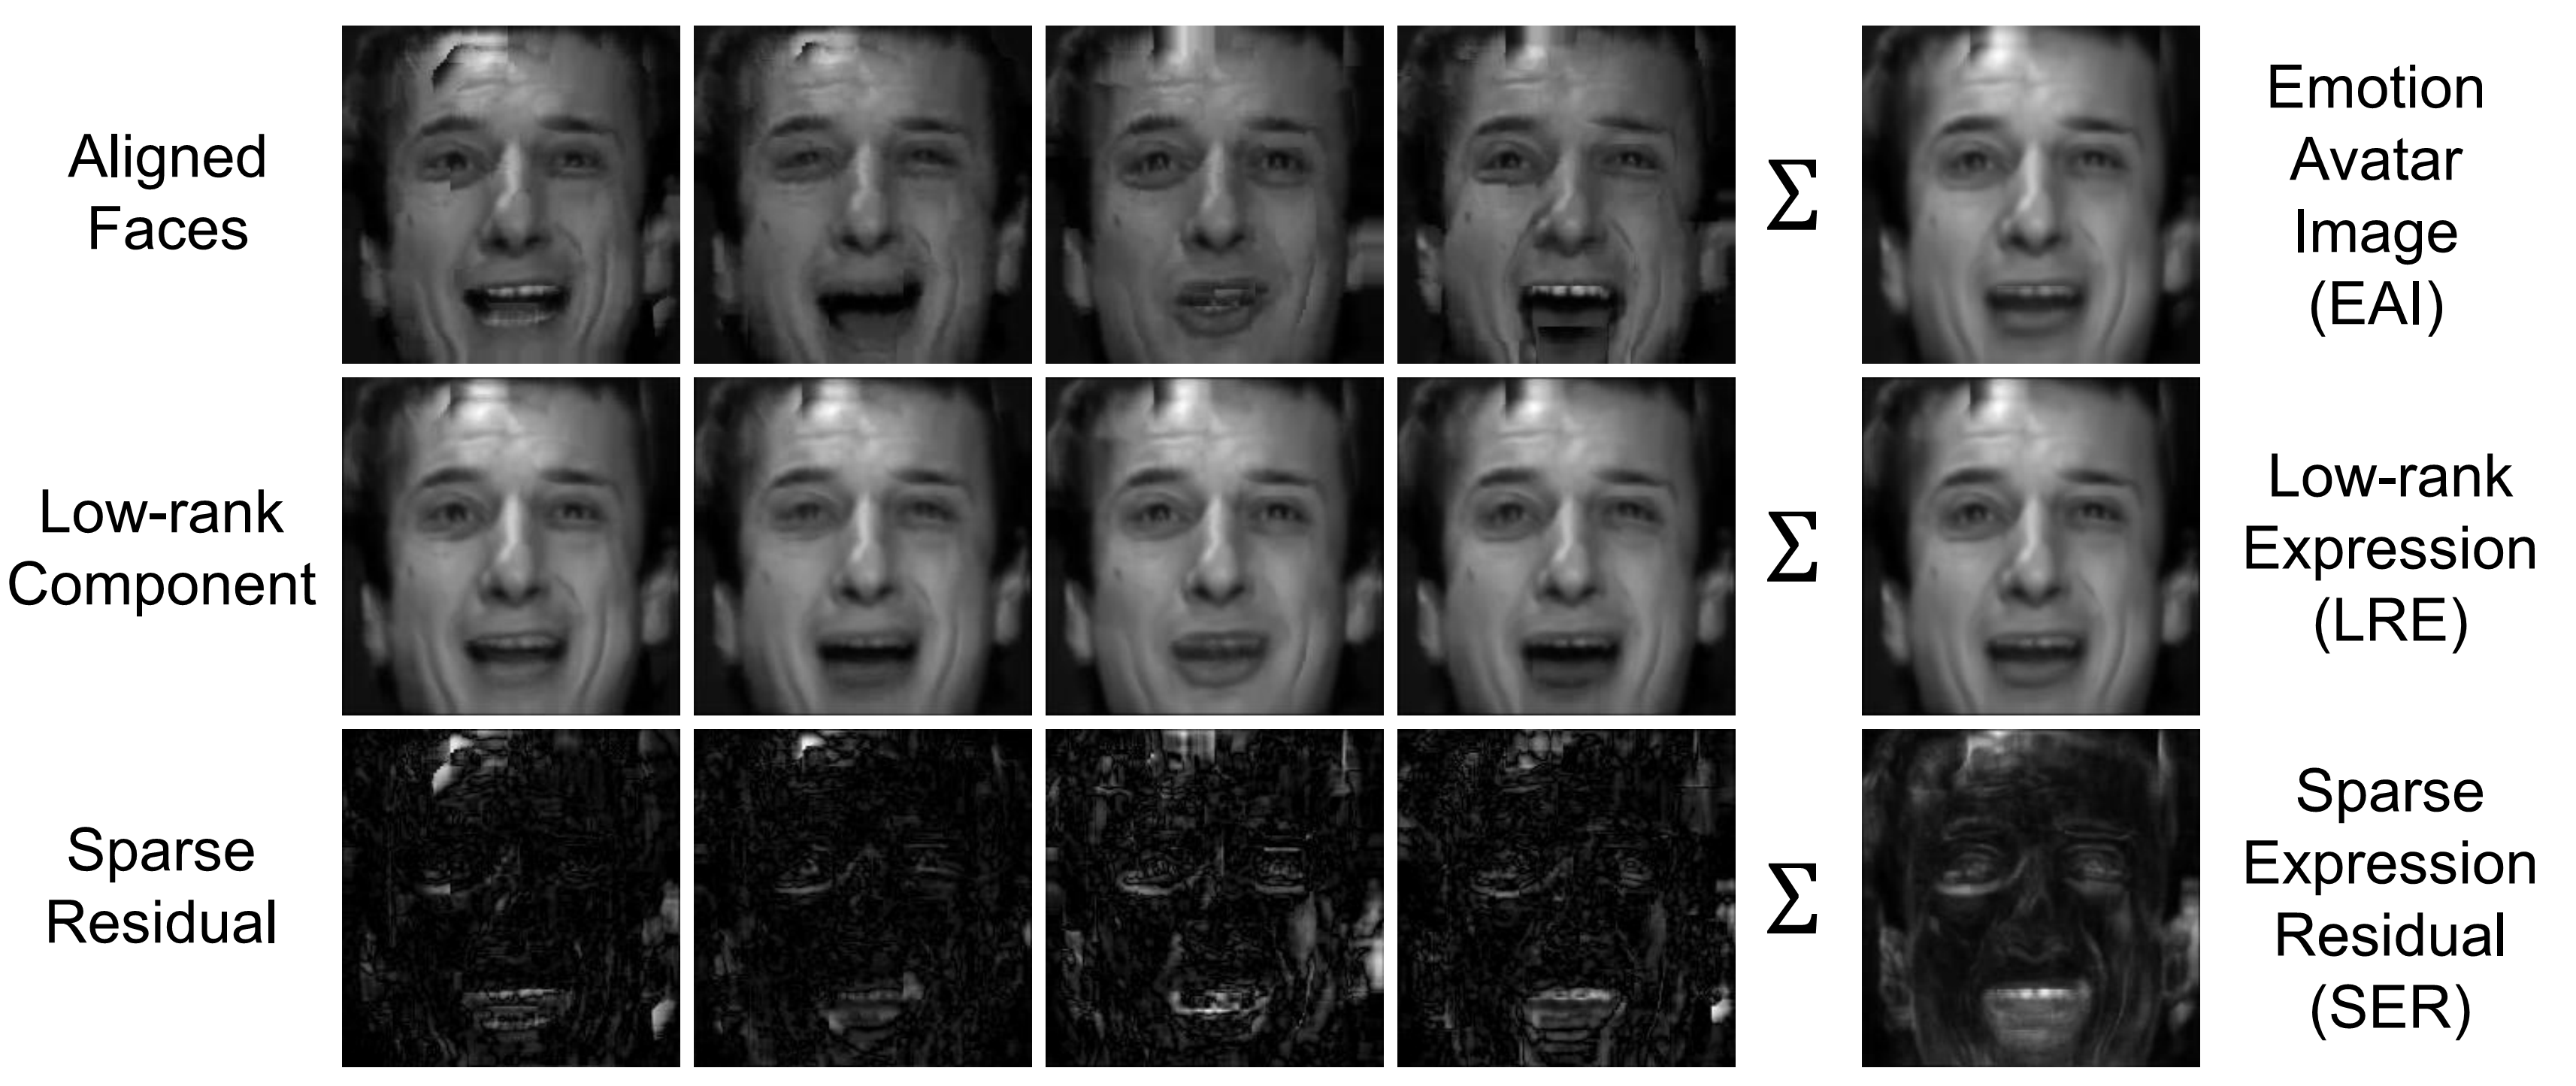
\includegraphics[width=\columnwidth]{pics/low_rank_sparse}
	\caption{The LRE and SER decomposition. A low-rank component and a sparse residual component are jointly estimated and decomposed from a sequence of aligned faces. Although individual frame differs from each other, the mean LRE visually resembles the EAI representation~\cite{Yang_SMCB12}.}
	\label{fig:low_rank_sparse}
\end{figure}

\subsection{Relation to Emotion Avatar Image (EAI) \label{sec:eai}}

EAI was proposed in~\cite{Yang_SMCB12} for the international competition on FERA Challenge~\cite{FERA11}. It is a robust image representation that summarizes facial expression videos and it generalizes well on person-independent expression recognition. The EAIs are iteratively generated along with the AR representation, which is canonical representation that captures the appearance of the entire dataset. The generalization of AR is also demonstrated in~\cite{Yang_SMCB12} such that the recognition performance is not degraded when AR is computed using outside datasets. As shown from row 1 of Fig.~\ref{fig:low_rank_sparse}, the EAI is computed from the mean of the aligned faces with respect to a certain level of AR (Level-1 in this case). It can be considered as a Maximum Likelihood (ML) estimate of the aligned sequences. 

On the other hand, the low-rank component and sparse residual of individual frame is recovered by Algorithm~\ref{alg}. As seen from row 2 of Fig.~\ref{fig:low_rank_sparse}, the low-rank components are jointly estimated from all frames of a sequence. Although individual frame appears to be different, its corresponding low-rank component resembles the ML estimate of the aligned faces, \textit{i.e.}, EAI (last column of Fig.~\ref{fig:low_rank_sparse}). More sample visualizations are shown in Fig.~\ref{fig:eai_lre_compare} for various sequences. 


\begin{figure}[htbp]
	\centering
		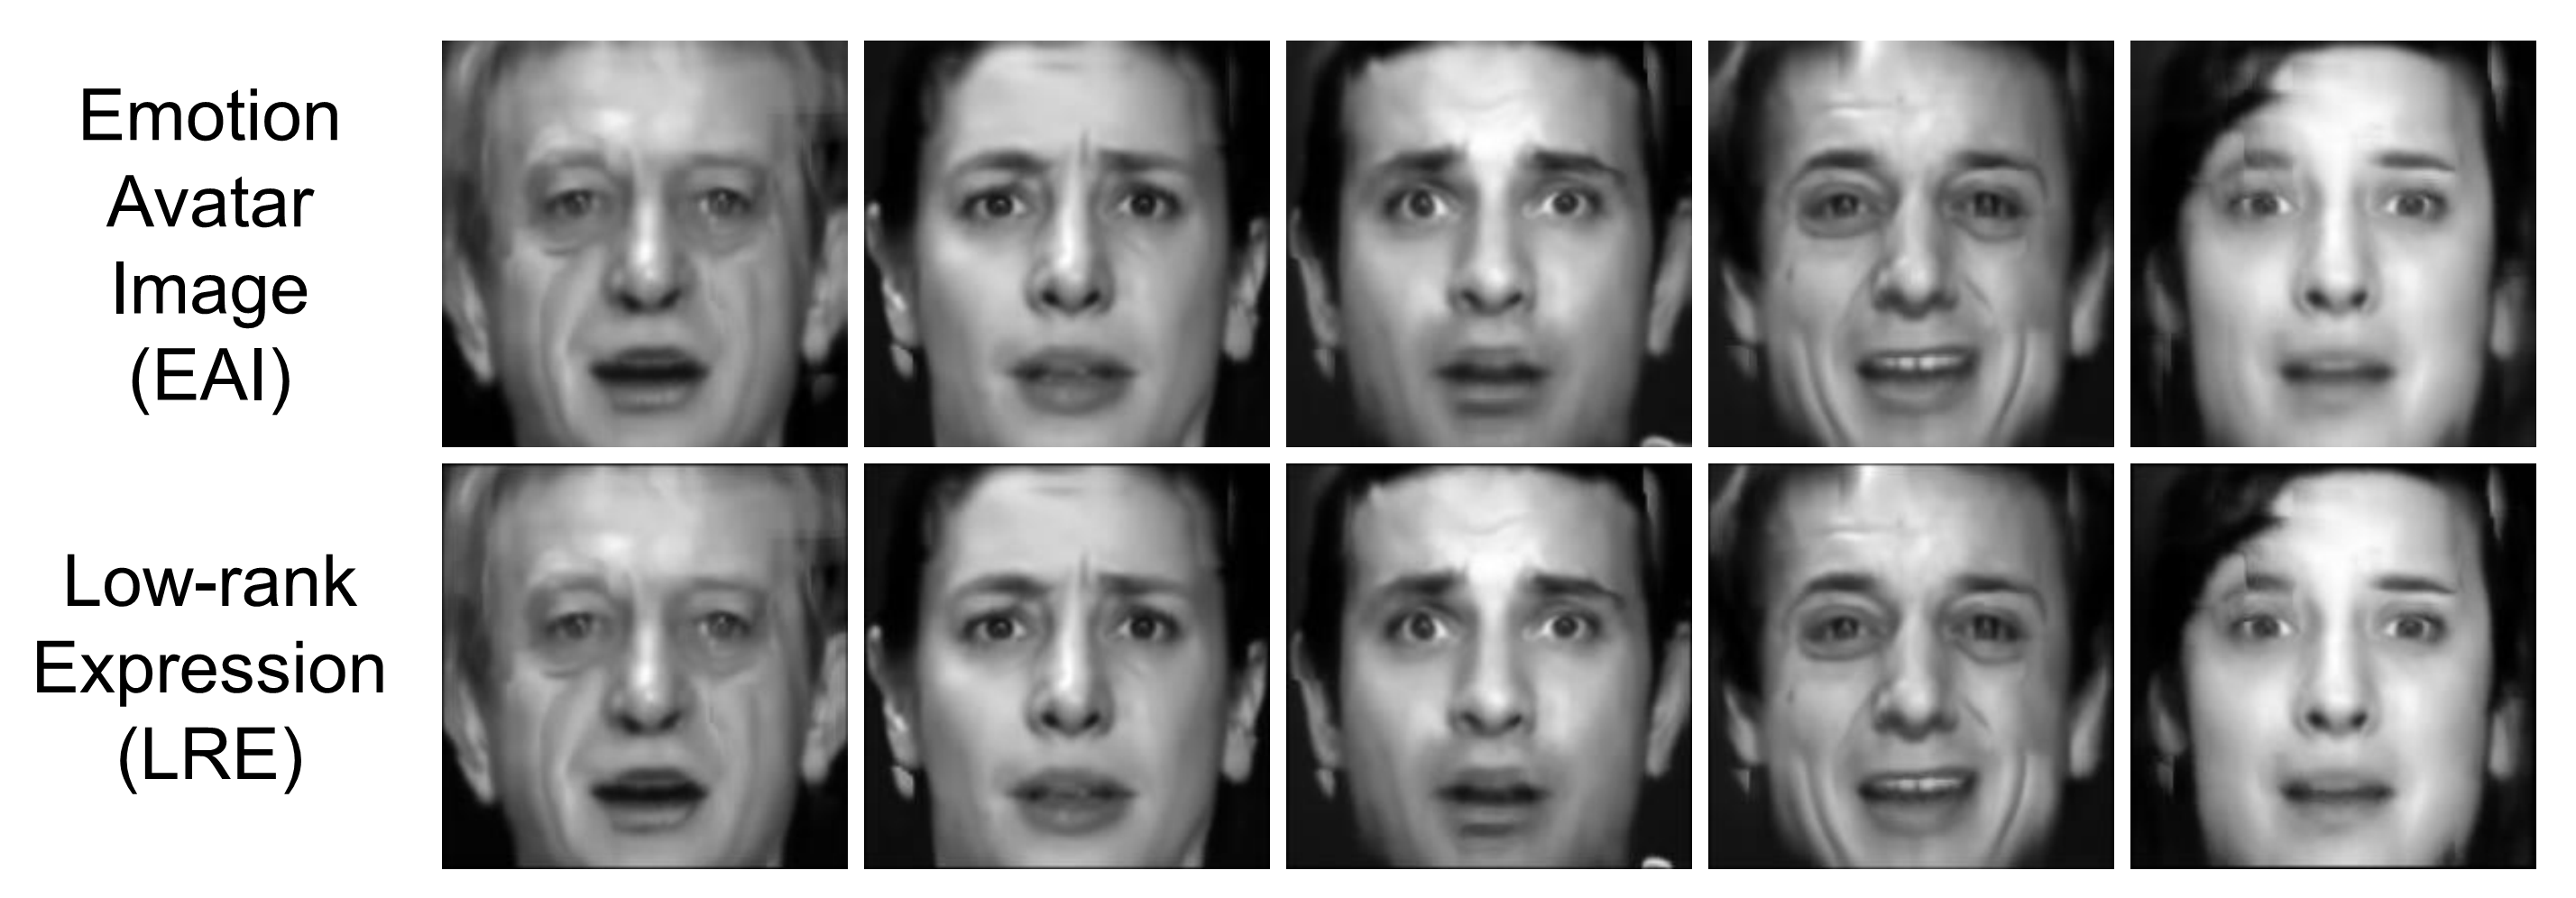
\includegraphics[width=\columnwidth]{pics/eai_lre_compare.png}
	\caption{The comparison of Low-Rank Expressions (LRE) and Emotion Avatar Images (EAI). Despite of being generated from different approaches, their appearances resemble each other at pixel level.}
	\label{fig:eai_lre_compare}
\end{figure}

As mentioned earlier, the expression appearance captured by the LRE reveals the underlining expression. For example, the expression \textit{Happiness} can be inferred from the LRE in Fig.~\ref{fig:low_rank_sparse} based on its lip corner expansion and cheek raise. However, LRE discards the expression dynamics of every individual. Fortunately, the sparse residual recovers the deviation of an aligned face from an LRE frame. Sparse residual models the subtle muscle motion of each particular frame from the underlining expression. 


\begin{figure*}[htbp]
\centering{
        \subfigure[The Low-Rank Expression (LRE) representations]{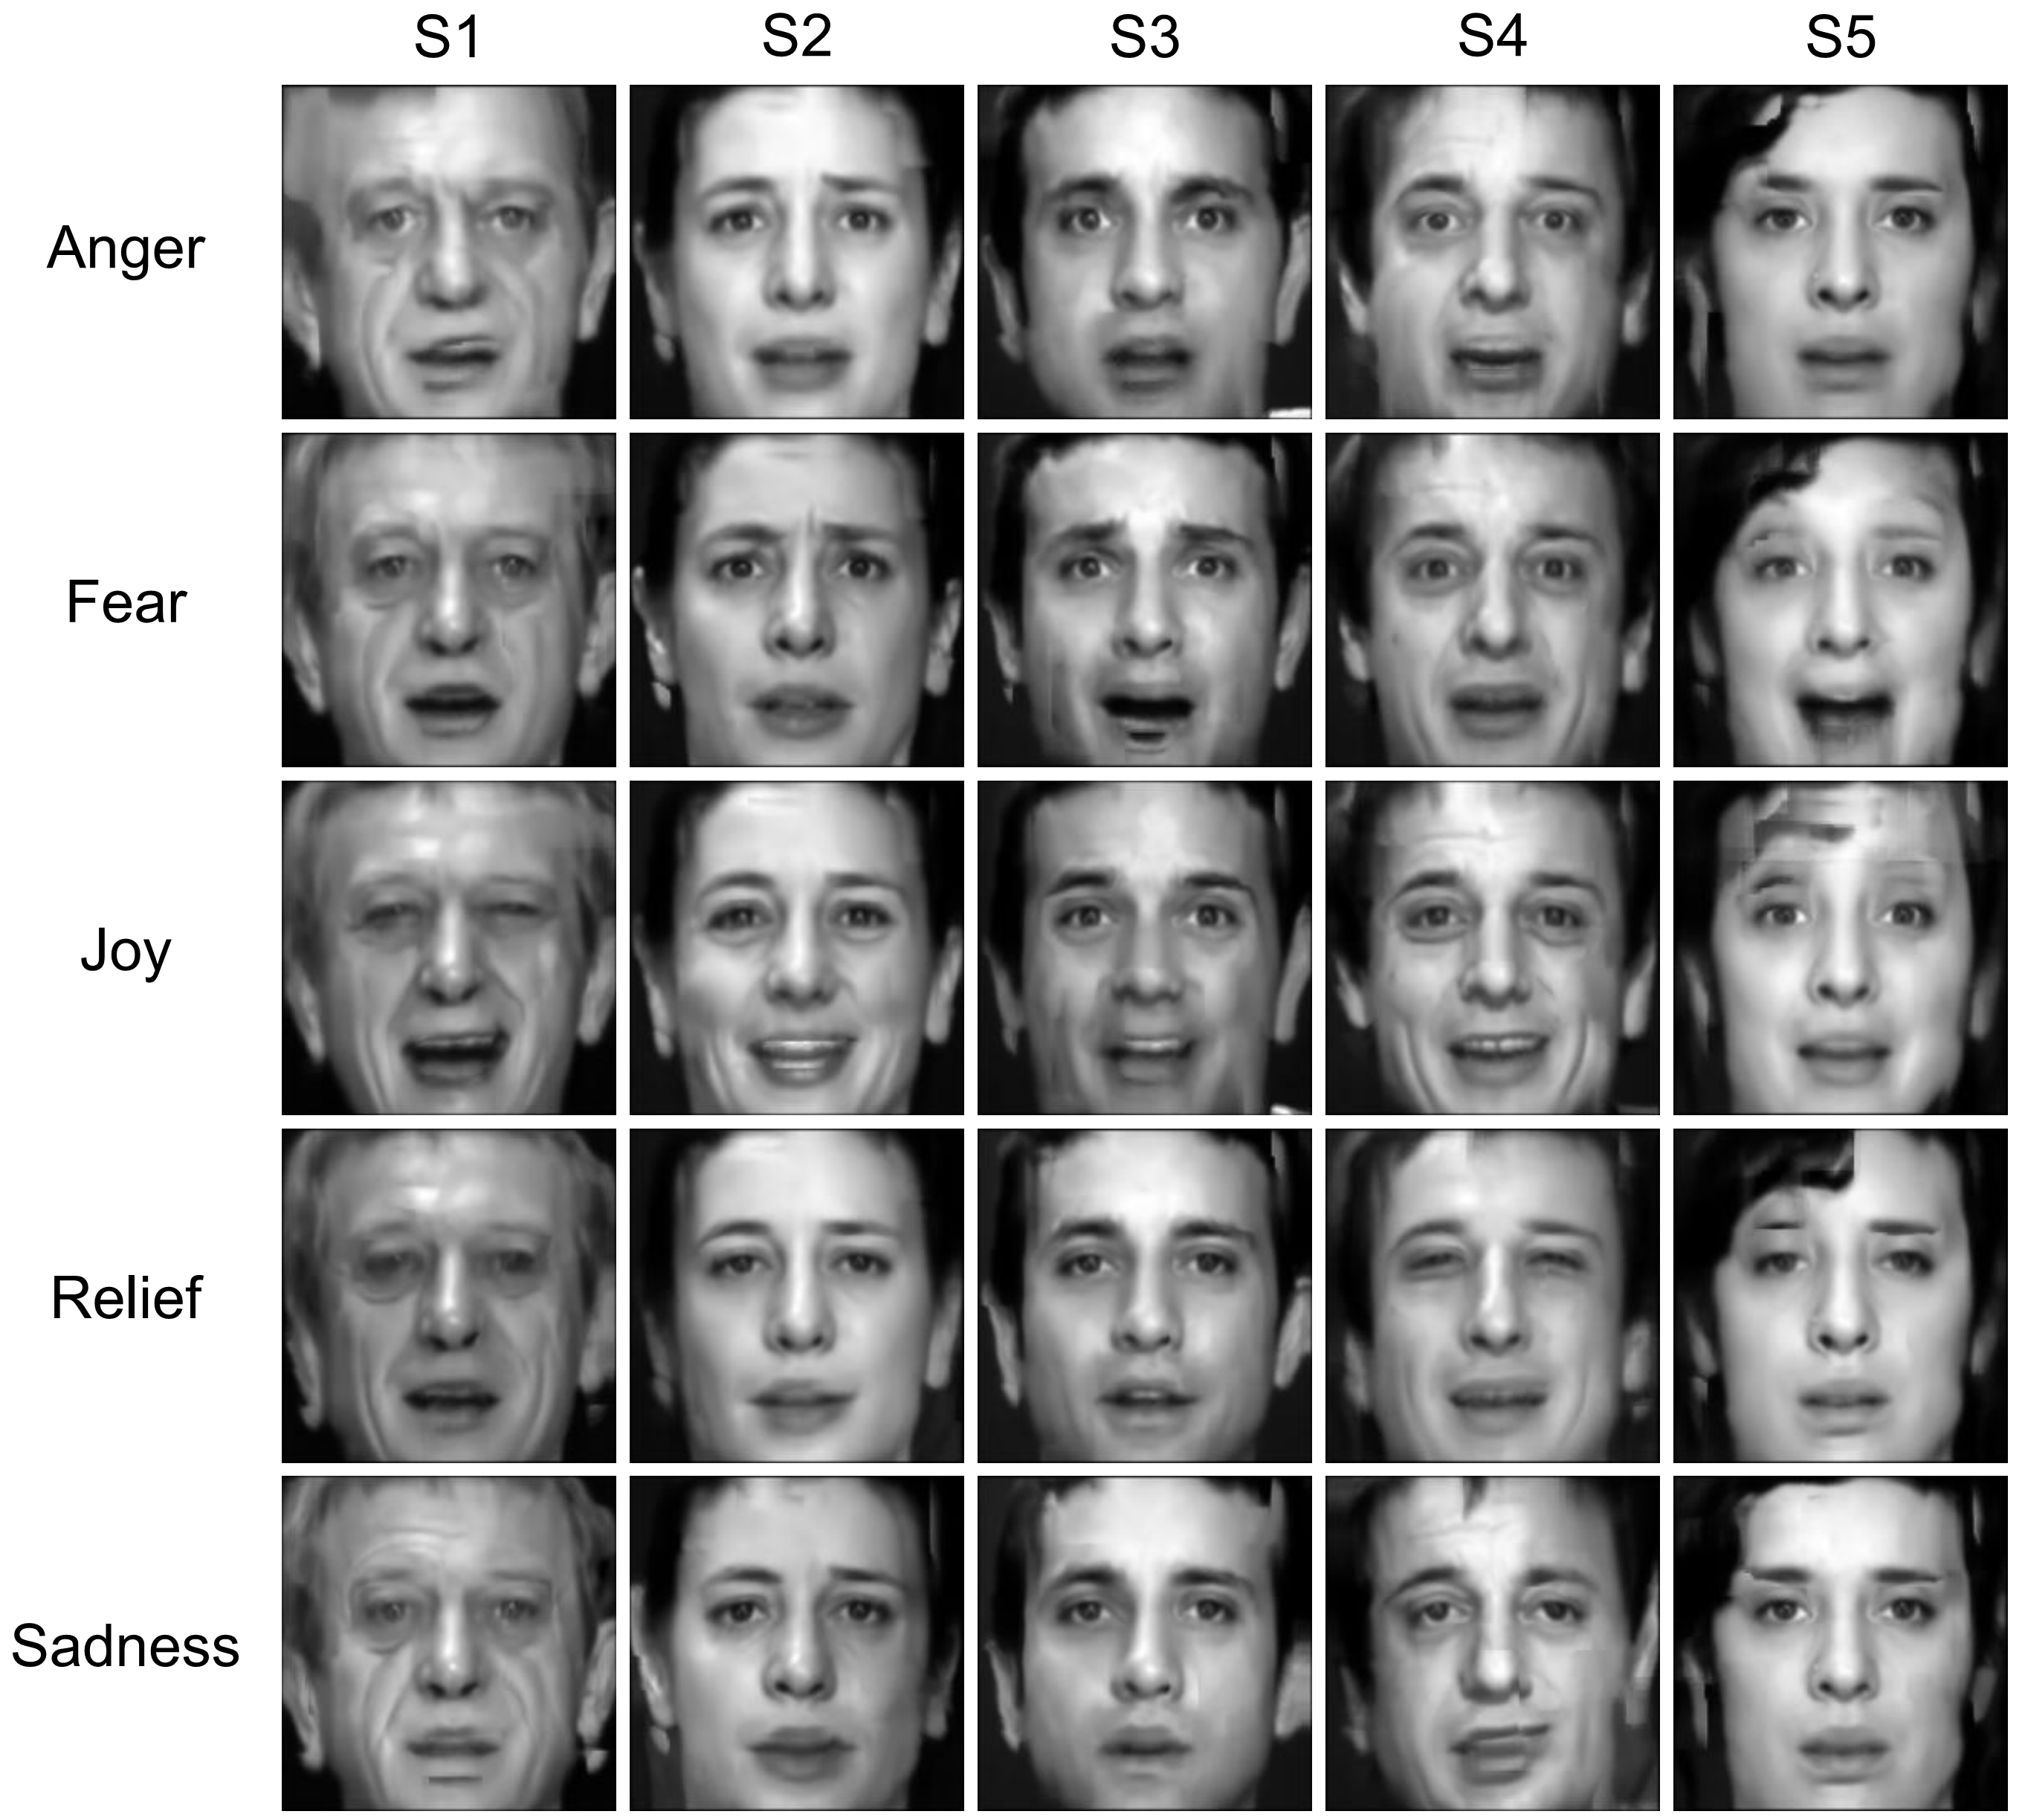
\includegraphics[width=0.45\linewidth]{pics/lre_vs_id.png}\label{fig:lre_vs_id}}
        \subfigure[The Sparse Residual Expression (SRE) representations]{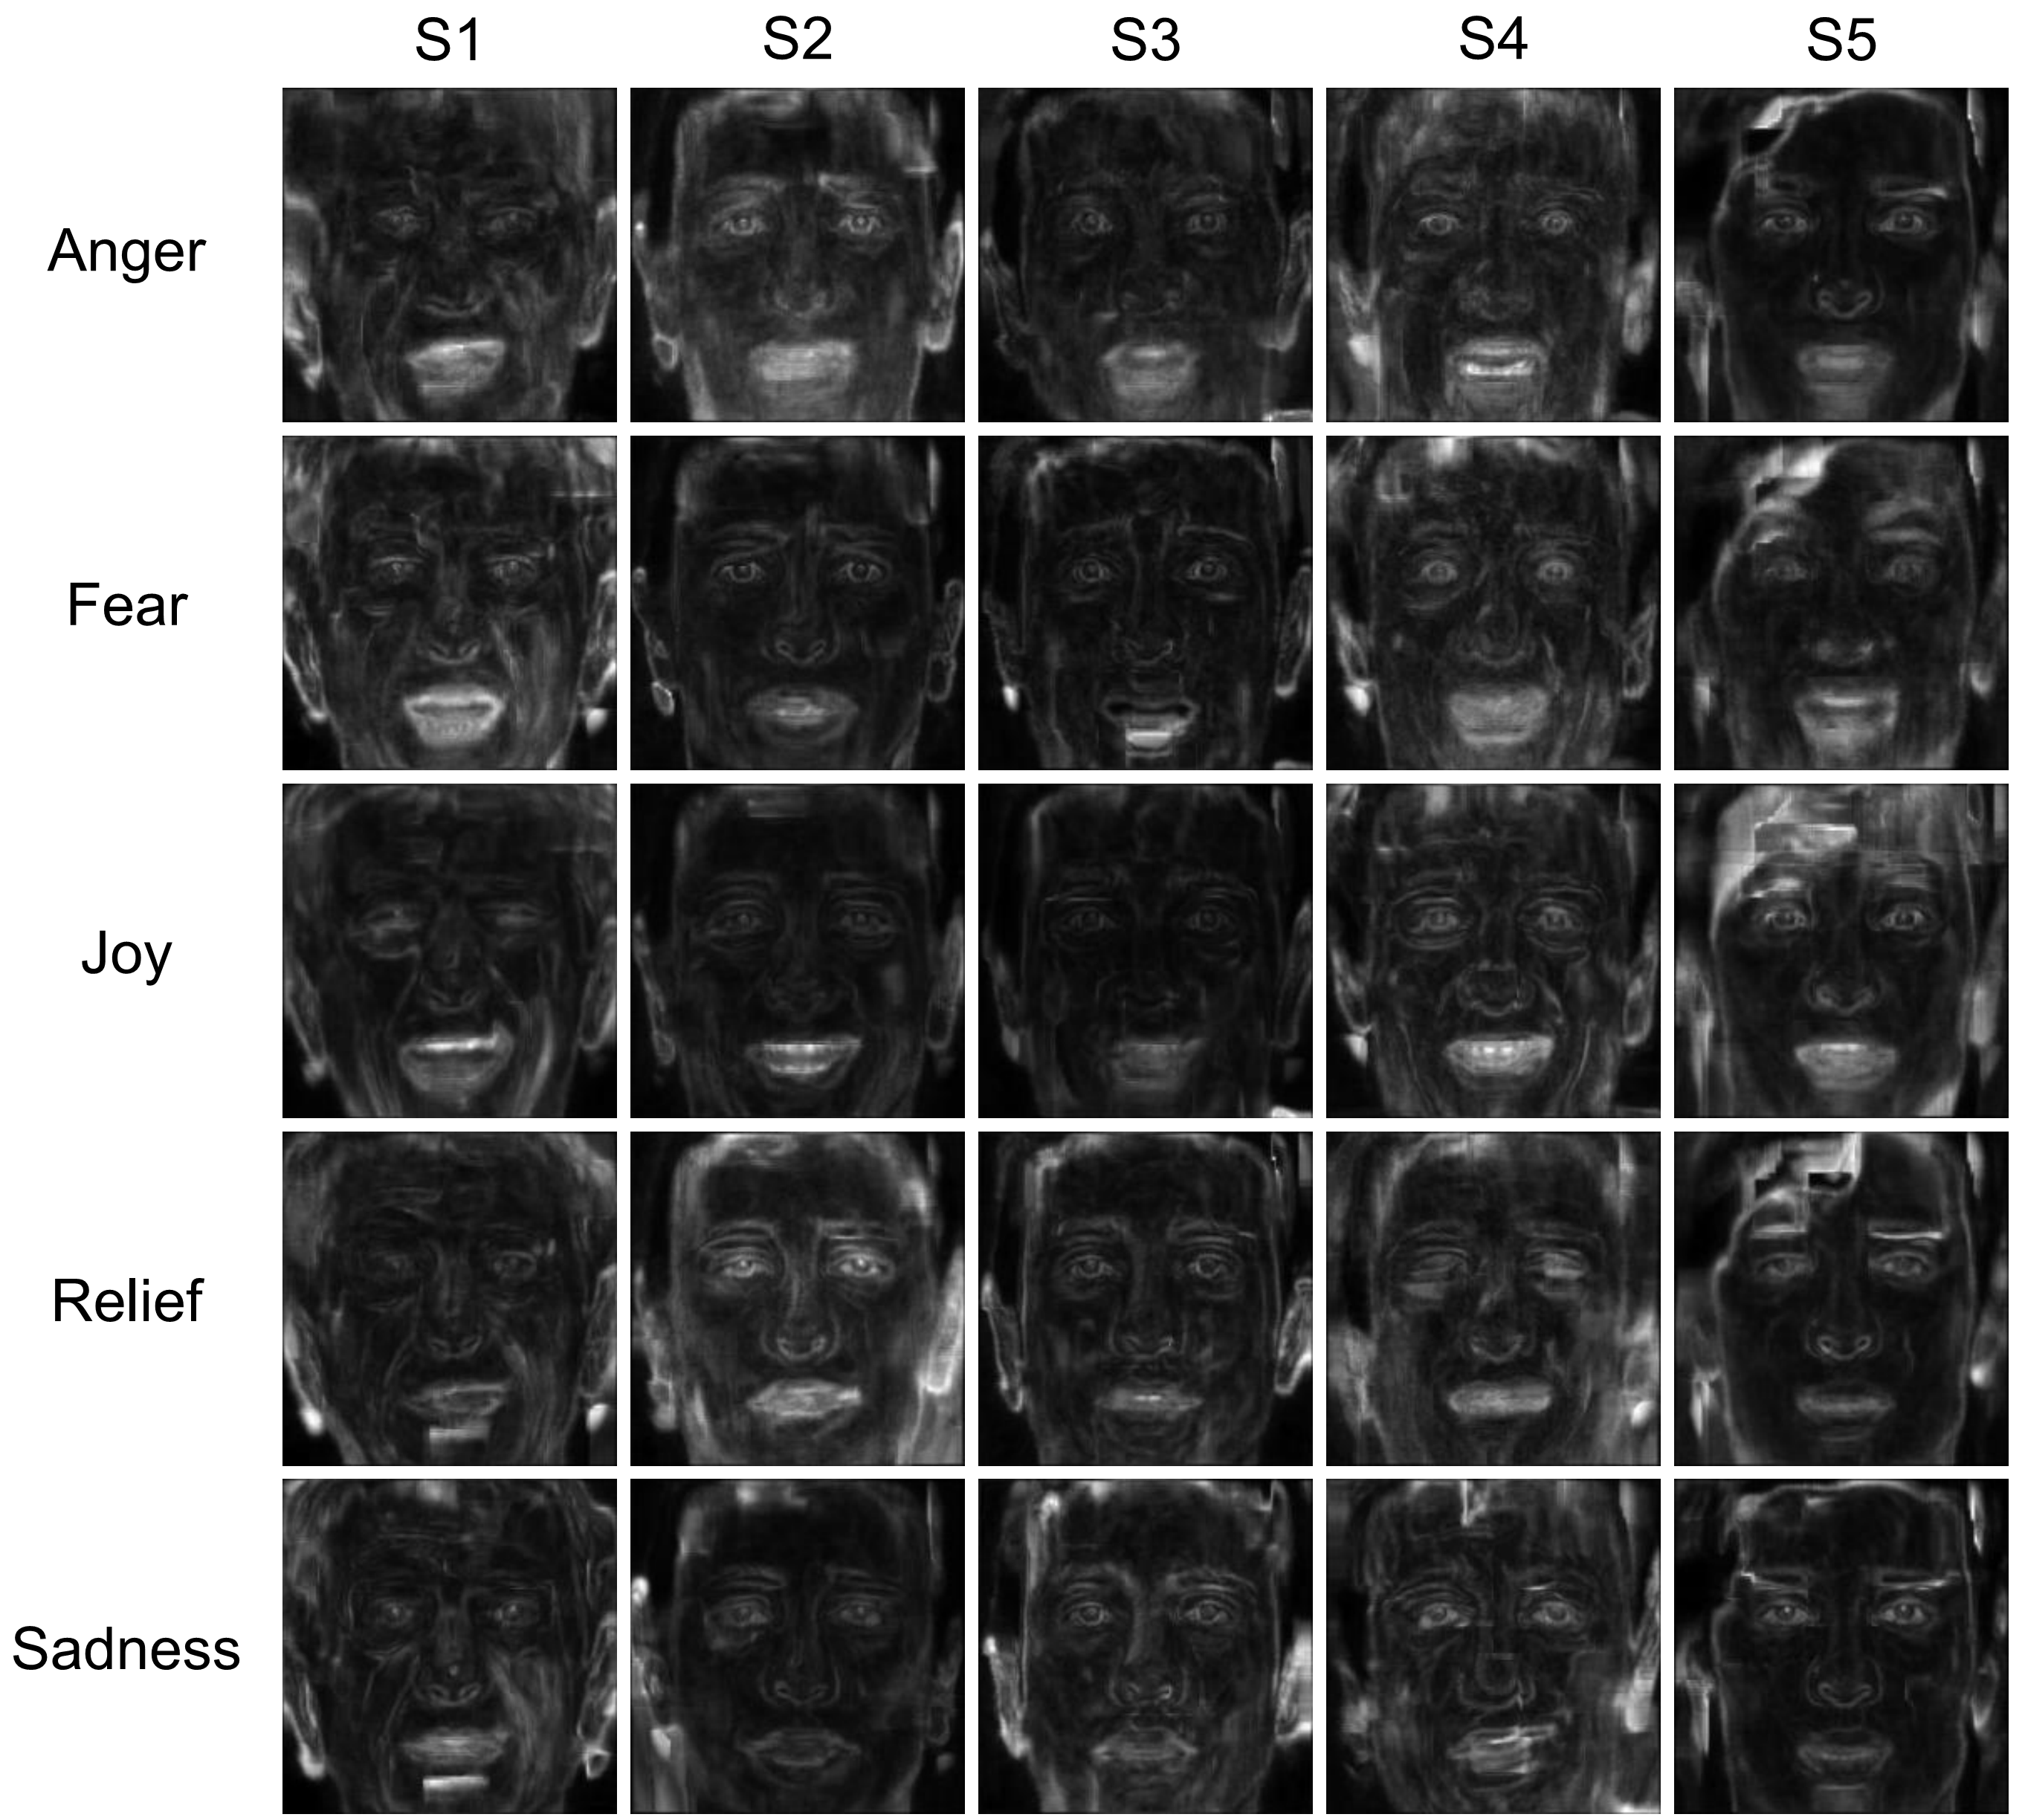
\includegraphics[width=0.45\linewidth]{pics/ser_vs_id.png}\label{fig:ser_vs_id}}
}
\caption{\label{fig:rep_vs_id} The sparse decomposition of a facial expression sequence. Each grid is an image representation of a video sequence. (a) The LRE representations. (b) The corresponding SRE representations.}
\end{figure*}

\section{Experimental Results\label{sec:exp}}

We conduct experiments on the \textit{uncontrolled} FERA-GEMEP dataset~\cite{FERA_data}. Qualitative results are first provided to visually demonstrate the validity of our method. The quantitative results then show that our method not only outperform the state-of-the-art approaches, but also has the potential for improvement with additional data. We also provide results on the \textit{controlled} CK+ dataset~\cite{CKplus}, for the completeness of the experiment.

\subsection{Experimental Setup}

After faces are detected from the sequences, we follow the standard image pre-processing steps in competing methods such as~\cite{Valstar12,Yang_SMCB12} for a better and fair comparison. The detected face images are resized to $200\times200$ pixels, and then divided into non-overlapping blocks of size $20\times20$. Texture features are extracted at each local block and then concatenated to form a final feature vector for classification. The feature extraction is conducted on both LRE and SER modalities, respectively. To prevent over-fitting, Principal Component Analysis (PCA) is carried out and the space with $99\%$ of the variation is retained for dimension reduction. 

For static features, the settings are the following:
\begin{enumerate}
\item LBP: the uniform LBP operator~\cite{Ojala_PAMI02} generates 59 basic patterns for a local patch. Given our region segmentation schema, the total feature dimension is $59\times 10\times 10=5900$. 
\item LPQ: we use the implementation described in~\cite{LPQ}. The feature size for each patch is $256$, yielding a feature dimension of $25600$ for $10 \times 10$ blocks. 
\end{enumerate}

For dynamic features, the settings are the following:
\begin{enumerate}
\item TOP-LBP: since the feature dimension enlarges by a multiple of $3$ compared with LBP, the total feature dimension is $3\times 5900=17700$.
\item TOP-LPQ: similar to TOP-LBP, for each sequence the TOP-LPQ feature dimension is $3\times 25600=76800$.  
\end{enumerate} 

In the following sections, we report results of various combinations of static and dynamic features on both LRE and SER representations. 


\begin{table}[!t]
\caption{The rank of person-independent test in FERA Challenge~\cite{Valstar12}\label{table:fera_team}}
\centering
\begin{tabular}{ll}
\toprule
	Teams~\ref{teams} & Accuracy \\ \midrule
	UCR 								& 0.75 \\ 
	UCSD-CERT						& 0.71 \\ 
	UIUC-UMC						& 0.66 \\ 
	KIT									& 0.66 \\ 
	ANU									& 0.65 \\ 
	NUS									& 0.64 \\ 
	QUT-CMU							& 0.62 \\ 
	UCL									& 0.61 \\ 
	UMont								& 0.58 \\ 
	MIT-Cambridge				& 0.45 \\ 
	Baseline						& 0.44 \\
\bottomrule
\end{tabular}
\end{table}

\subsection{Uncontrolled Data: FERA-GEMEP Dataset}

The FERA-GEMEP~\cite{FERA_data} is an uncontrolled facial expression dataset, \textit{i.e.}, in the process of data collection, subjects are asked to convey one of the following five emotions at a time: \textit{Anger}, \textit{Fear}, \textit{Joy}, \textit{Relief}, and \textit{Sadness}, without any control of their head or body movement. Each video segment contains one subject displaying expressions that correspond to one emotion. The average video length is about 2 seconds with 30 frames per second (FPS). Most subjects are uttering some meaningless phrases while displaying expressions, and there are 3 to 5 videos for each subject with the same emotion. All experiments in this paper are designed to be \textit{person-independent} (\textit{i.e.}, no testing subject is included in the training set), in order to validate the generalization ability of the proposed algorithm. 

The original FERA-GEMEP data contain a training and a testing set, where there are 7 subjects (3 males and 4 females) in the training set, and 6 subjects (3 males and 3 females) in the testing set. The facial expression videos of both sets are provided and the expression label is only available for the training set. The participants can use other publicly available data in addition to FERA training set for training. The predictions on the test set are submitted to the FERA organizer for an independent evaluation. Table~\ref{table:fera_team} shows the challenge participants\footnote{\label{teams}Teams are ranked based on the FERA Challenge person-independent test. \textbf{UCR}: University of California at Riverside; \textbf{UCSD-CERT}: University of California at San Diego; \textbf{UIUC-UMC}: University of Illinois at Urbana-Champaign; University of Missouri; \textbf{KIT}: Karlsruhe Institute of Technology; \textbf{ANU}: Australian National University; \textbf{NUS}: National University of Singapore; \textbf{QUT-CMU}: Queensland University of Technology; Carnegie Mellon University; \textbf{UCL}: University College London; \textbf{UMont.}: University of Montreal;  \textbf{MIT-Cambridge}: Massachusetts Institute of Technology; University of Cambridge.} and the corresponding person-independent test results.


Since the ground truth labels are only available for the training set, we evaluate our algorithm using this set. Note that although our results are not directly comparable to those in Table~\ref{table:fera_team}, we compare our method with the best performer in Table~\ref{table:fera_team}, \textit{i.e.}, EAI~\cite{Yang_SMCB12}, under the protocol of this paper. Specifically, we carry out leave-one-subject-out cross-validation using both static and dynamic features extracted from the LREs and SREs and these features are evaluated both individually and jointly. Fig.~\ref{fig:rep_vs_id} provides a visualization of the mean LRE and SRE representations of sample expression videos of various subjects for all emotion categories in the training set. The classification results are shown in Table~\ref{table:comp_lbp} and Table~\ref{table:comp_lpq}, respectively. The symbol ``--'' means a particular module is not used for feature extraction. In addition, we report the results of the best performing approach~\cite{Yang_SMCB12} in FERA challenge as a baseline comparison with same settings. We should address that unlike most of the other methods which use additional training data, this work and~\cite{Yang_SMCB12} solely rely on the FERA training set. 

Several interesting findings can be observed from the results in Table~\ref{table:comp_lbp} and Table~\ref{table:comp_lpq}. \textit{First}, the performance using static features on LRE only is on par with the EAI representation in~\cite{Yang_SMCB12}, $0.68$ for LBP and $0.7$ for LPQ. This is congruent with our qualitative analysis in Section~\ref{sec:eai} such that EAI and mean LRE have very similar appearance. \textit{Second}, when considering single module performance, LRE results are consistently higher than SER ones (for both static and dynamic feature using both LBP and LPQ), which means LREs are more discriminative than SERs. This shows that if only single module is to be considered, global structure of a facial expression is more informative than its local muscle motion. \textit{Third}, combining both module almost always improves the recognition performance. For example, in Table~\ref{table:comp_lpq}, single module performances for LRE and SER using LPQ features are $0.7$ and $0.62$, respectively. Combining both modules improves the accuracy to $0.75$, which demonstrates that the information captured by both modules complements each other and improved results are obtained by exploiting the local muscle motion. \textit{Fourth}, incorporating dynamic features further improves the performance. The best performance is achieved when dynamic features are extracted from both the LRE and SER modules. This informs us that the person-independent modeling is an effective strategy, which not only diminishes the person-specific information, but also provides a reasonable means for dynamic feature extraction. 

The confusion matrix for the best-performance setting, \textit{i.e.}, LRE+SER with TOP-LPQ, is tabulated in Table.~\ref{table:mat_fera}. \textit{Anger} and \textit{Fear} are misclassified to each other more often because the global structure of these two expressions are more similar compared with other expressions. This is qualitatively demonstrated in Fig.~\ref{fig:lre_vs_id}, where the appearance of the first two rows resemble each other more than other rows. It is also shown in~\cite{Valstar12} that \textit{Fear} is indeed the most challenging case for this dataset. However, incorporating local muscle dynamics helps better characterizing the \textit{Fear} expression. 


%\begin{table}[htbp]
%\caption{The accuracy comparison of our approach to the best performance system in the FERA Challenge\label{table:comp}}
%\begin{center}
%\begin{tabular}{|c|c|c|c|c|c|}
%\toprule
	%Approach 									& TOP-LPQ	& TOP-LBP 	& LPQ 	& LBP 	& Gabor \\ \midrule
	%LRE+SER										& \textbf{0.78} 		& 0.72 	& 0.76 	&	0.73	& 0.68	\\
	%UCR	\cite{Yang_SMCB12}		& 0.70 		& 0.67 	& \textbf{0.71} 	& 0.68	& 0.66	\\ 
	%LRE												& \textbf{0.72} 		& 0.66 	& 0.70 	& 0.68	& 0.66	\\
	%SER												& \textbf{0.65} 		& 0.65 	& 0.62 	& 0.60	& 0.55	\\
%\bottomrule
%\end{tabular}
%\end{center}
%\end{table}


\begin{table}[!t]
\caption{Classification accuracy on FERA-GEMEP dataset using LBP\label{table:comp_lbp}}
\centering
\scriptsize
\begin{tabular}{l|l|l||l|l|l}
\toprule
LRE & SER & Accuracy	& LRE	& SER	& Accuracy \\ \midrule 
LBP	& --		& 0.68	& -- & LBP & 0.6 \\
TOP-LBP & -- & 0.67 & -- & TOP-LBP & 0.62 \\
LBP & LBP & 0.7 & LBP & TOP-LBP & 0.72 \\
TOP-LBP & LBP & 0.7 & TOP-LBP & TOP-LBP & \textbf{0.73} \\ \midrule
\multicolumn{2}{l}{UCR~\cite{Yang_SMCB12}: LBP} & 0.68 & \multicolumn{2}{l}{UCR~\cite{Yang_SMCB12}: TOP-LBP} & 0.69 \\
\bottomrule

\end{tabular}
\end{table}


\begin{table}[!t]
\caption{Classification accuracy on FERA-GEMEP dataset using LPQ\label{table:comp_lpq}}
\centering
\scriptsize
\begin{tabular}{l|l|l||l|l|l}
\toprule
LRE & SER & Accuracy	& LRE	& SER	& Accuracy \\ \midrule 
LPQ	& --		& 0.7	& -- & LPQ & 0.62 \\
TOP-LPQ & -- & 0.72 & -- & TOP-LPQ & 0.65 \\
LPQ & LPQ & 0.75 & LPQ & TOP-LPQ & 0.77 \\
TOP-LPQ & LPQ & 0.76 & TOP-LPQ & TOP-LPQ & \textbf{0.78} \\ \midrule
\multicolumn{2}{l}{UCR~\cite{Yang_SMCB12}: LPQ} & 0.7 & \multicolumn{2}{l}{UCR~\cite{Yang_SMCB12}: TOP-LPQ} & 0.73 \\
\bottomrule

\end{tabular}
\end{table}




\begin{table}[htbp]
\caption{confusion matrix for the FERA training dataset using LER+SER.
(An=Anger, Fe=Fear, Jo=Joy, Re=Relief, Sa=Sadness)}
\begin{center}
\label{table:mat_fera}
\begin{tabular}{c|c|ccccc|}
\multicolumn{7}{c}{True Label} \\ \cline{2-7}
\multirow{7}{*}{\begin{sideways}Prediction\end{sideways}} && An & Fe & Jo & Re & Sa \\ \cline{2-7}
&An				&\textbf{62.1} &13.2  &4.8  &3.6  &   \\ 
&Fe       &16.4  &\textbf{71.4}  &3.2   &1.8   & \\ 
&Jo       &7.5  &5.5   &\textbf{85.5} &3.6  &    \\ 
&Re       &5.8   &1.8   &4.8   &\textbf{78.4} &8.6    \\ 
&Sa       &8.2   &8.1   &1.6  &12.5 &\textbf{91.4}  \\ \cline{2-7}
&Average  &\multicolumn{5}{c|}{\textbf{77.8}} \\ \cline{2-7}

\end{tabular}
\end{center}
\end{table}


To thoroughly evaluate our approach, we carry out more experiments with analysis. Unless mentioned otherwise, the following analysis uses this best-performing setting. 

\textbf{Effect of Training Size with a Fixed Subject Pool:} we observe that the performance of EAI (\textit{i.e.}, $0.7$ as shown in Table~\ref{table:comp_lpq}) is inferior to that in the FERA challenge~\cite{Yang_SMCB12} (\textit{i.e.}, $0.75$ as shown in Table~\ref{table:fera_team}). We believe that this is due to a smaller training size in our person-independent experimental setting. To verify this hypothesis, we carried out a leave-one-subject-out cross-validation with respect to different training sizes using various representations. For a specific training set size, we randomly select the training data according to person-independent constraint from the subject pool to train a classifier. This experiment is repeated for 10 times for each training set size, and the average classification rate is reported in Fig.~\ref{fig:effect_training_size}. 

\begin{figure}[!h]
	\centering
		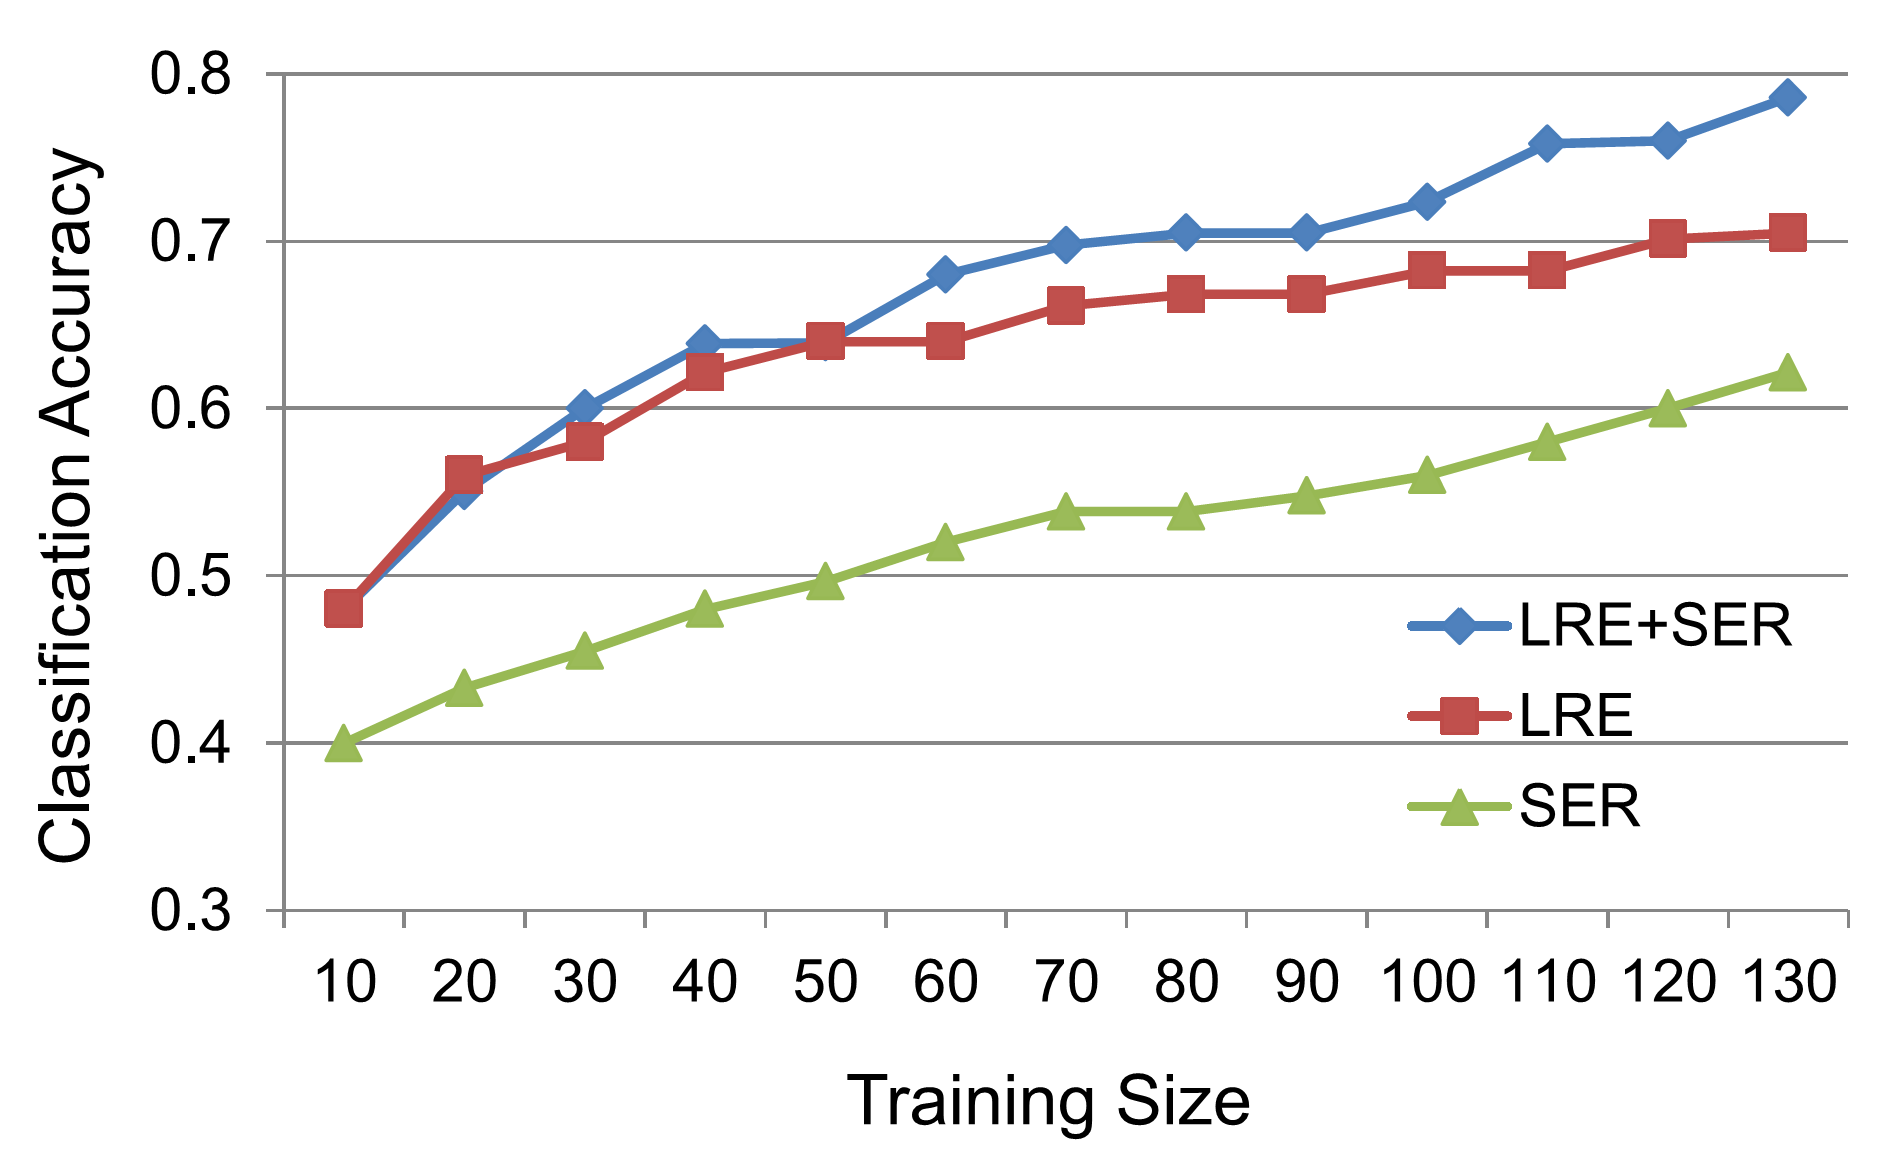
\includegraphics[width=.9\columnwidth]{pics/effect_training_size.png}
	\caption{The person-independent recognition accuracy with various training size from a fixed subject pool. The feature in use is TOP-LPQ. The performance of LRE is spurred by the additional information captured in SER.}
	\label{fig:effect_training_size}
\end{figure}

As seen in Fig.~\ref{fig:effect_training_size}, the classification rate steadily raises as the training set size increases for all three curves. This informs us that given more training data from the same training subject pool, the performance improves. Additionally, it is observed that the increase rate for LRE+SER, especially when training size becomes larger. This demonstrates that the SER indeed captures more discriminative facial muscle motion for expression recognition and provides useful and complementary information to LRE. The performance of LRE+SER is not saturated as the training size reaches the maximum (130 in this experiment), suggesting a potential performance gain using more data.




\textbf{Effect of Subject Pool Size:} under a person-independent setting, it is also interesting to discover the impact of the number of subjects in the training set. Thus, for each leave-one-subject-out test using LRE+SER, we vary the number of subjects, $k$, in training from 1 to 6 (since there are 7 subjects in the dataset), and conduct the test for ${6 \choose k}$ times. For example, when 2 subjects are in the training, there can be ${6 \choose 2}=15$ possible combinations of subjects, we record the test results for all combinations. Fig.~\ref{fig:effect_people_num} shows an increasing trend for recognition accuracy as the number of subjects in training increases. This shows that the performance is likely to be improved as the number of training subjects increases. In addition, the decreasing variance of the classification accuracy can be observed, suggesting a more stable performance as the training subjects pool grows. 


\begin{figure}[htbp]
	\centering
		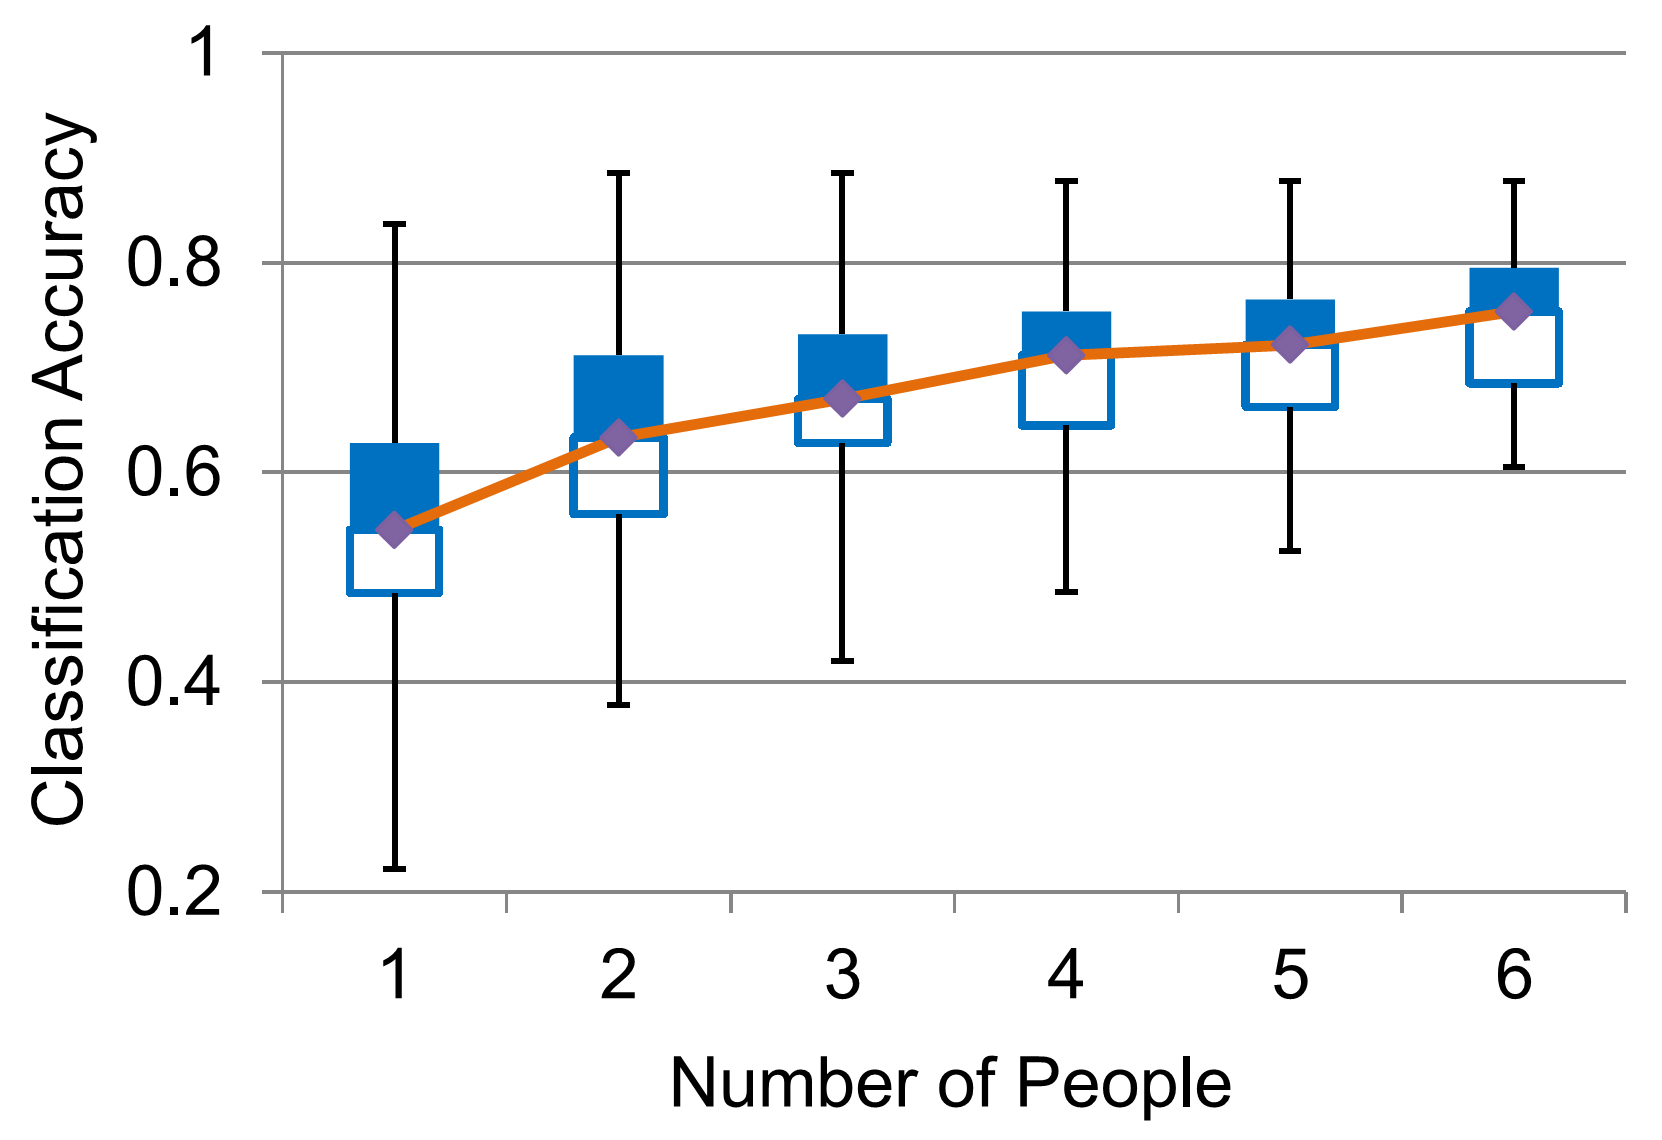
\includegraphics[width=.75\columnwidth]{pics/effect_people_num.png}
	\caption{The boxplot of person-independent recognition accuracy using LRE+SER and TOP-LPQ with various number of people in the training set. The mean performance at the second quartile are connected to illustrate the trend. In general, the performance increases and becomes more stable when the number of training subjects grows.}
	\label{fig:effect_people_num}
\end{figure}


\subsection{Controlled Data: CK+ dataset}

The Extended Cohn-Kanade dataset (CK+)~\cite{CKplus} is a facial expression dataset with 7 categories of expressions, namely, \textit{Anger}, \textit{Contempt}, \textit{Disgust}, \textit{Fear}, \textit{Happy}, \textit{Sadness}, and \textit{Surprise}. This is a controlled dataset since the subjects constrained their head pose on purpose, and the expression displayed always follows the ``neutral-onset-apex" pattern. These explicit control may not only hide the true muscle contraction of an expression, but also changes the expression dynamics~\cite{Bartlett03,Ekman2005}. Although the philosophy of our algorithm is not designed for this fully controlled data, for rigorous validation of our method, we also carry out person-independent tests and evaluate our LRE+SER representation using LPQ features on 316 sequences from 123 subjects in this dataset. LPQ with same setting is chosen for a better comparison with the other methods. 

\begin{table}[htbp]
\caption{confusion matrix for CK+ dataset using LER+SER.
(An=Anger, Co=Contempt, Di=Disgust, Fe=Fear, Ha=Happy, Sa=Sadness, Su=Surprise)}
\begin{center}
\label{table:CK_result}
\begin{tabular}{c|c|ccccccc|}

\multicolumn{9}{c}{True Label} \\ \cline{2-9}
\multirow{8}{*}{\begin{sideways}Prediction\end{sideways}} && An & Co & Di & Fe & Ha & Sa & Su \\ \cline{2-9}
&An          &\textbf{75} &22.2  &1.8  &8  &  &25.9 &  \\ 
&Co       &2.3  &\textbf{72.2}  &   &   &  &3.7  &1.2 \\ 
&Di        &4.5  &   &\textbf{94.6} &  &1.6 &3.7 &2.4  \\ 
&Fe           &2.3   &   &   &\textbf{68} &  &3.7  &1.2  \\ 
&Ha          &4.5   &   &1.8  &8 &\textbf{96.8} &  &  \\ 
&Sa        &9.1  &  &  &4   &  &\textbf{48.1} & \\ 
&Su       &2.3  &5.6 &1.8  &12 &1.6  &14.8 &\textbf{95.2} \\ \cline{2-9}
&Average &\multicolumn{7}{c|}{\textbf{85.1}} \\ \cline{2-9}

\end{tabular}
\end{center}
\end{table}


As seen in confusion matrix in Table~\ref{table:CK_result}, the LRE+SER representation achieves $85.1\%$ accuracy on average, outperforming an accuracy of $82.6\%$ by EAI reported in~\cite{Yang_SMCB12}. This again demonstrates that the information captured by the SER improves the expression recognition accuracy. The algorithm in~\cite{Zhao_PAMI07} using the same dynamic texture feature, has a better performance on CK+ dataset. We believe it is because the experiment in~\cite{Zhao_PAMI07} was designed with 10-fold cross validation. Although there is no subject that displays the same expression twice in CK+, this experiment setting does not strictly exclude testing subject in the training set. On the contrary, our experimental design is strictly person-independent.

Besides, the CK+ data has only one or a few apex expression for each ``neutral-onset-apex" sequence. This unrealistic setting reduces the intensity of the expression captured by LREs, which appears to be more neutral compared with the mean LRE of FERA-GEMEP data. Fig.~\ref{fig:ck_eai} shows a visualization of mean LRE representations for sample sequences from the CK+ dataset. 

\begin{figure}[htbp]
	\centering
		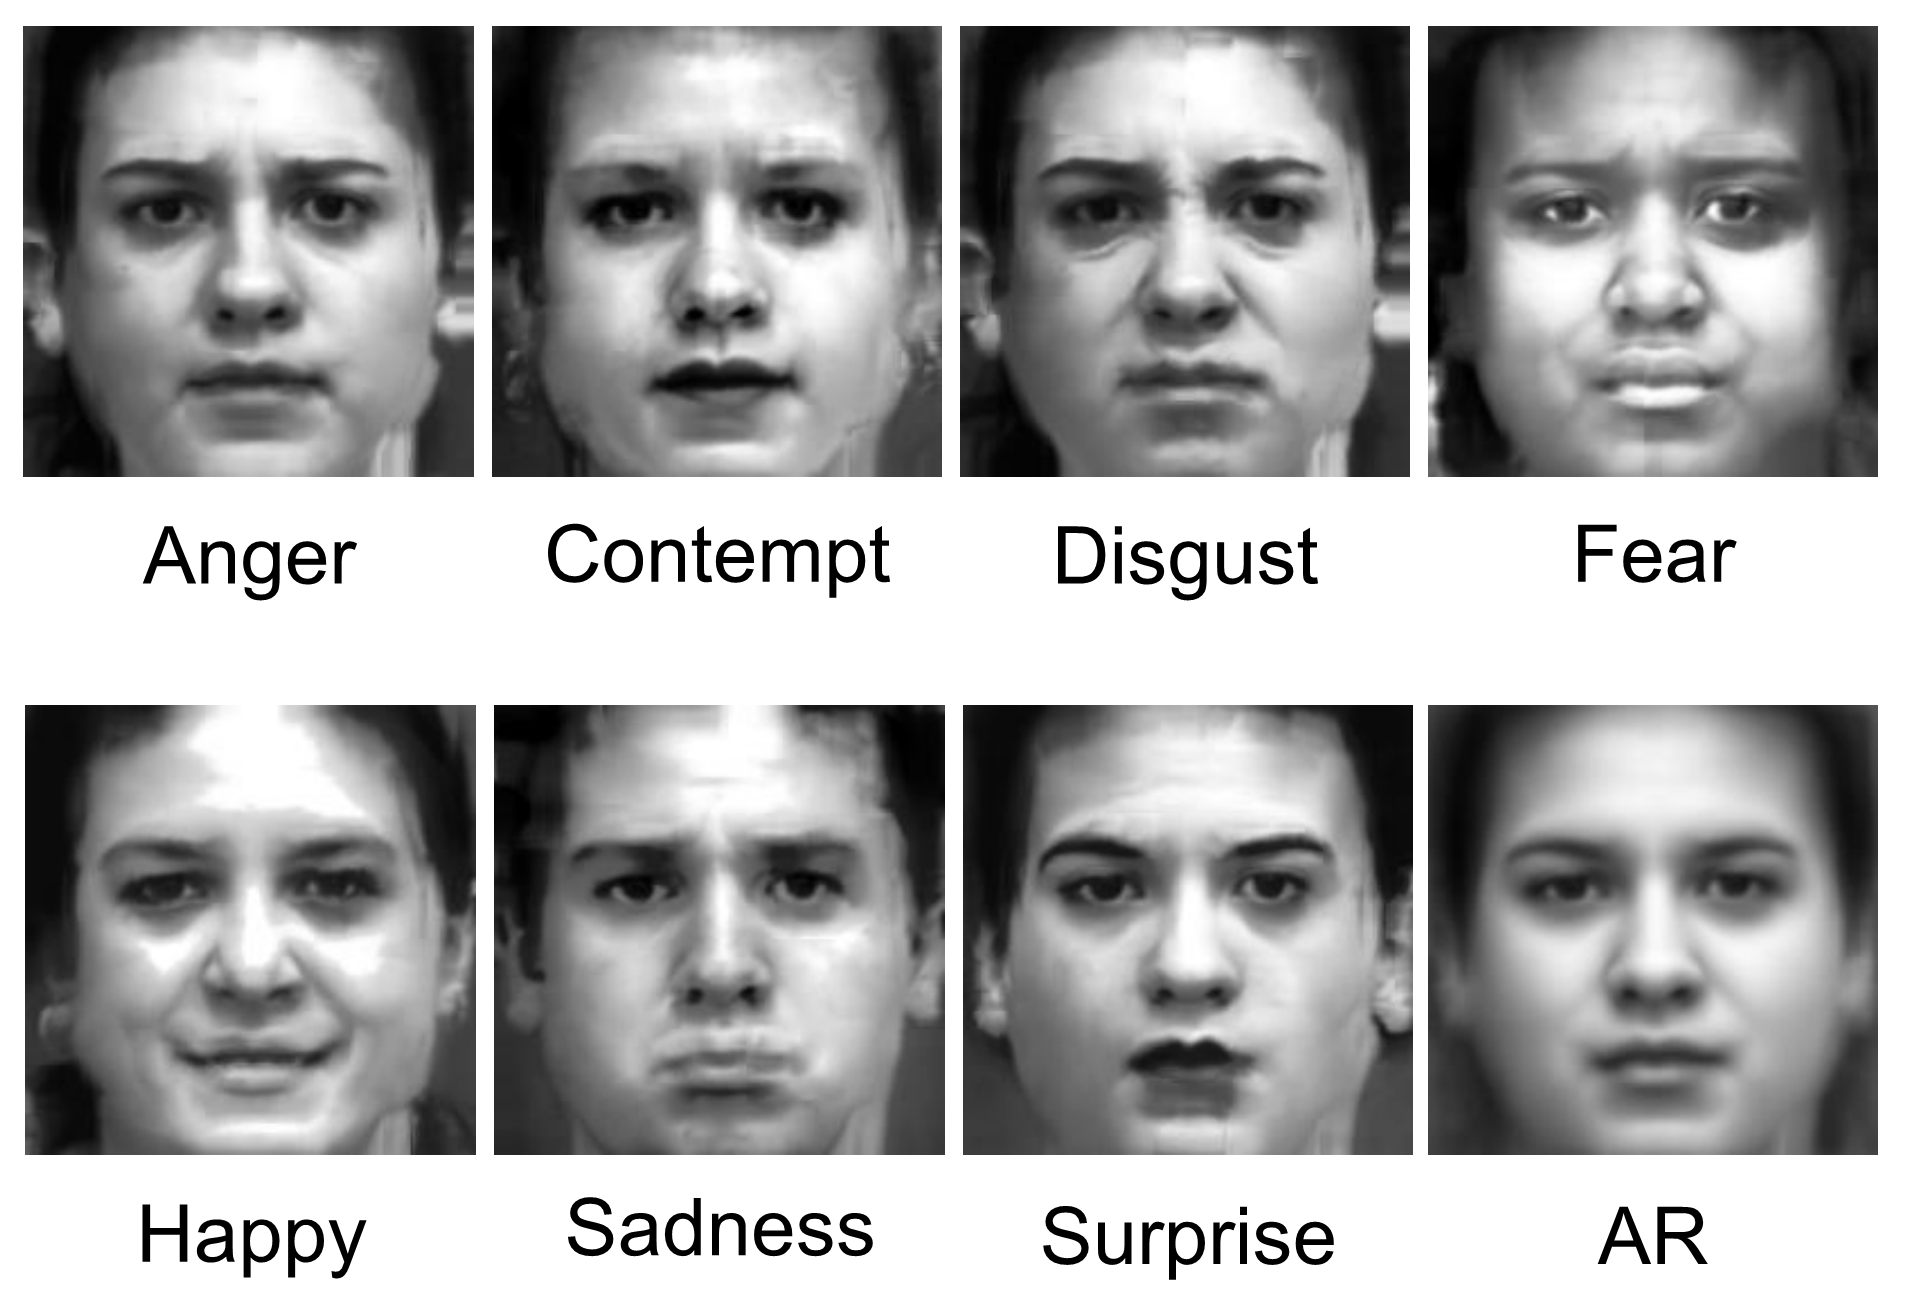
\includegraphics[width=.7\columnwidth]{pics/ck_eai.png}
	\caption{Sample mean LRE representations from the CK+ dataset. The lower right grid shows the Avatar Reference generated from~\cite{Yang_SMCB12}. Although the person-specific information is attenuated as the appearance of different subjects visually resemble each other, the discriminative expression information is hidden and difficult to be distinguished. In general, they appear to be more ``neutral'' compared with the mean LRE representations of the sequences in FERA-GEMEP dataset as shown in Fig.~\ref{fig:lre_vs_id}.}
	\label{fig:ck_eai}
\end{figure}


In addition, through a diagnostic experiment, we have found that the classification performance has a strong correlation with the training size for each class category, as shown in Fig.~\ref{fig:fig_ck_size}. We plot the classification accuracy along with the training set size for each category in Fig.~\ref{fig:fig_ck_size}. The categories such as \textit{Disgust}, \textit{Happy}, and \textit{Surprise}, which have more training data, achieve a much higher accuracy. This also shows the potential of improvement for our algorithm given more training samples for the under-performing categories. 


\begin{figure}[htbp]
	\centering
		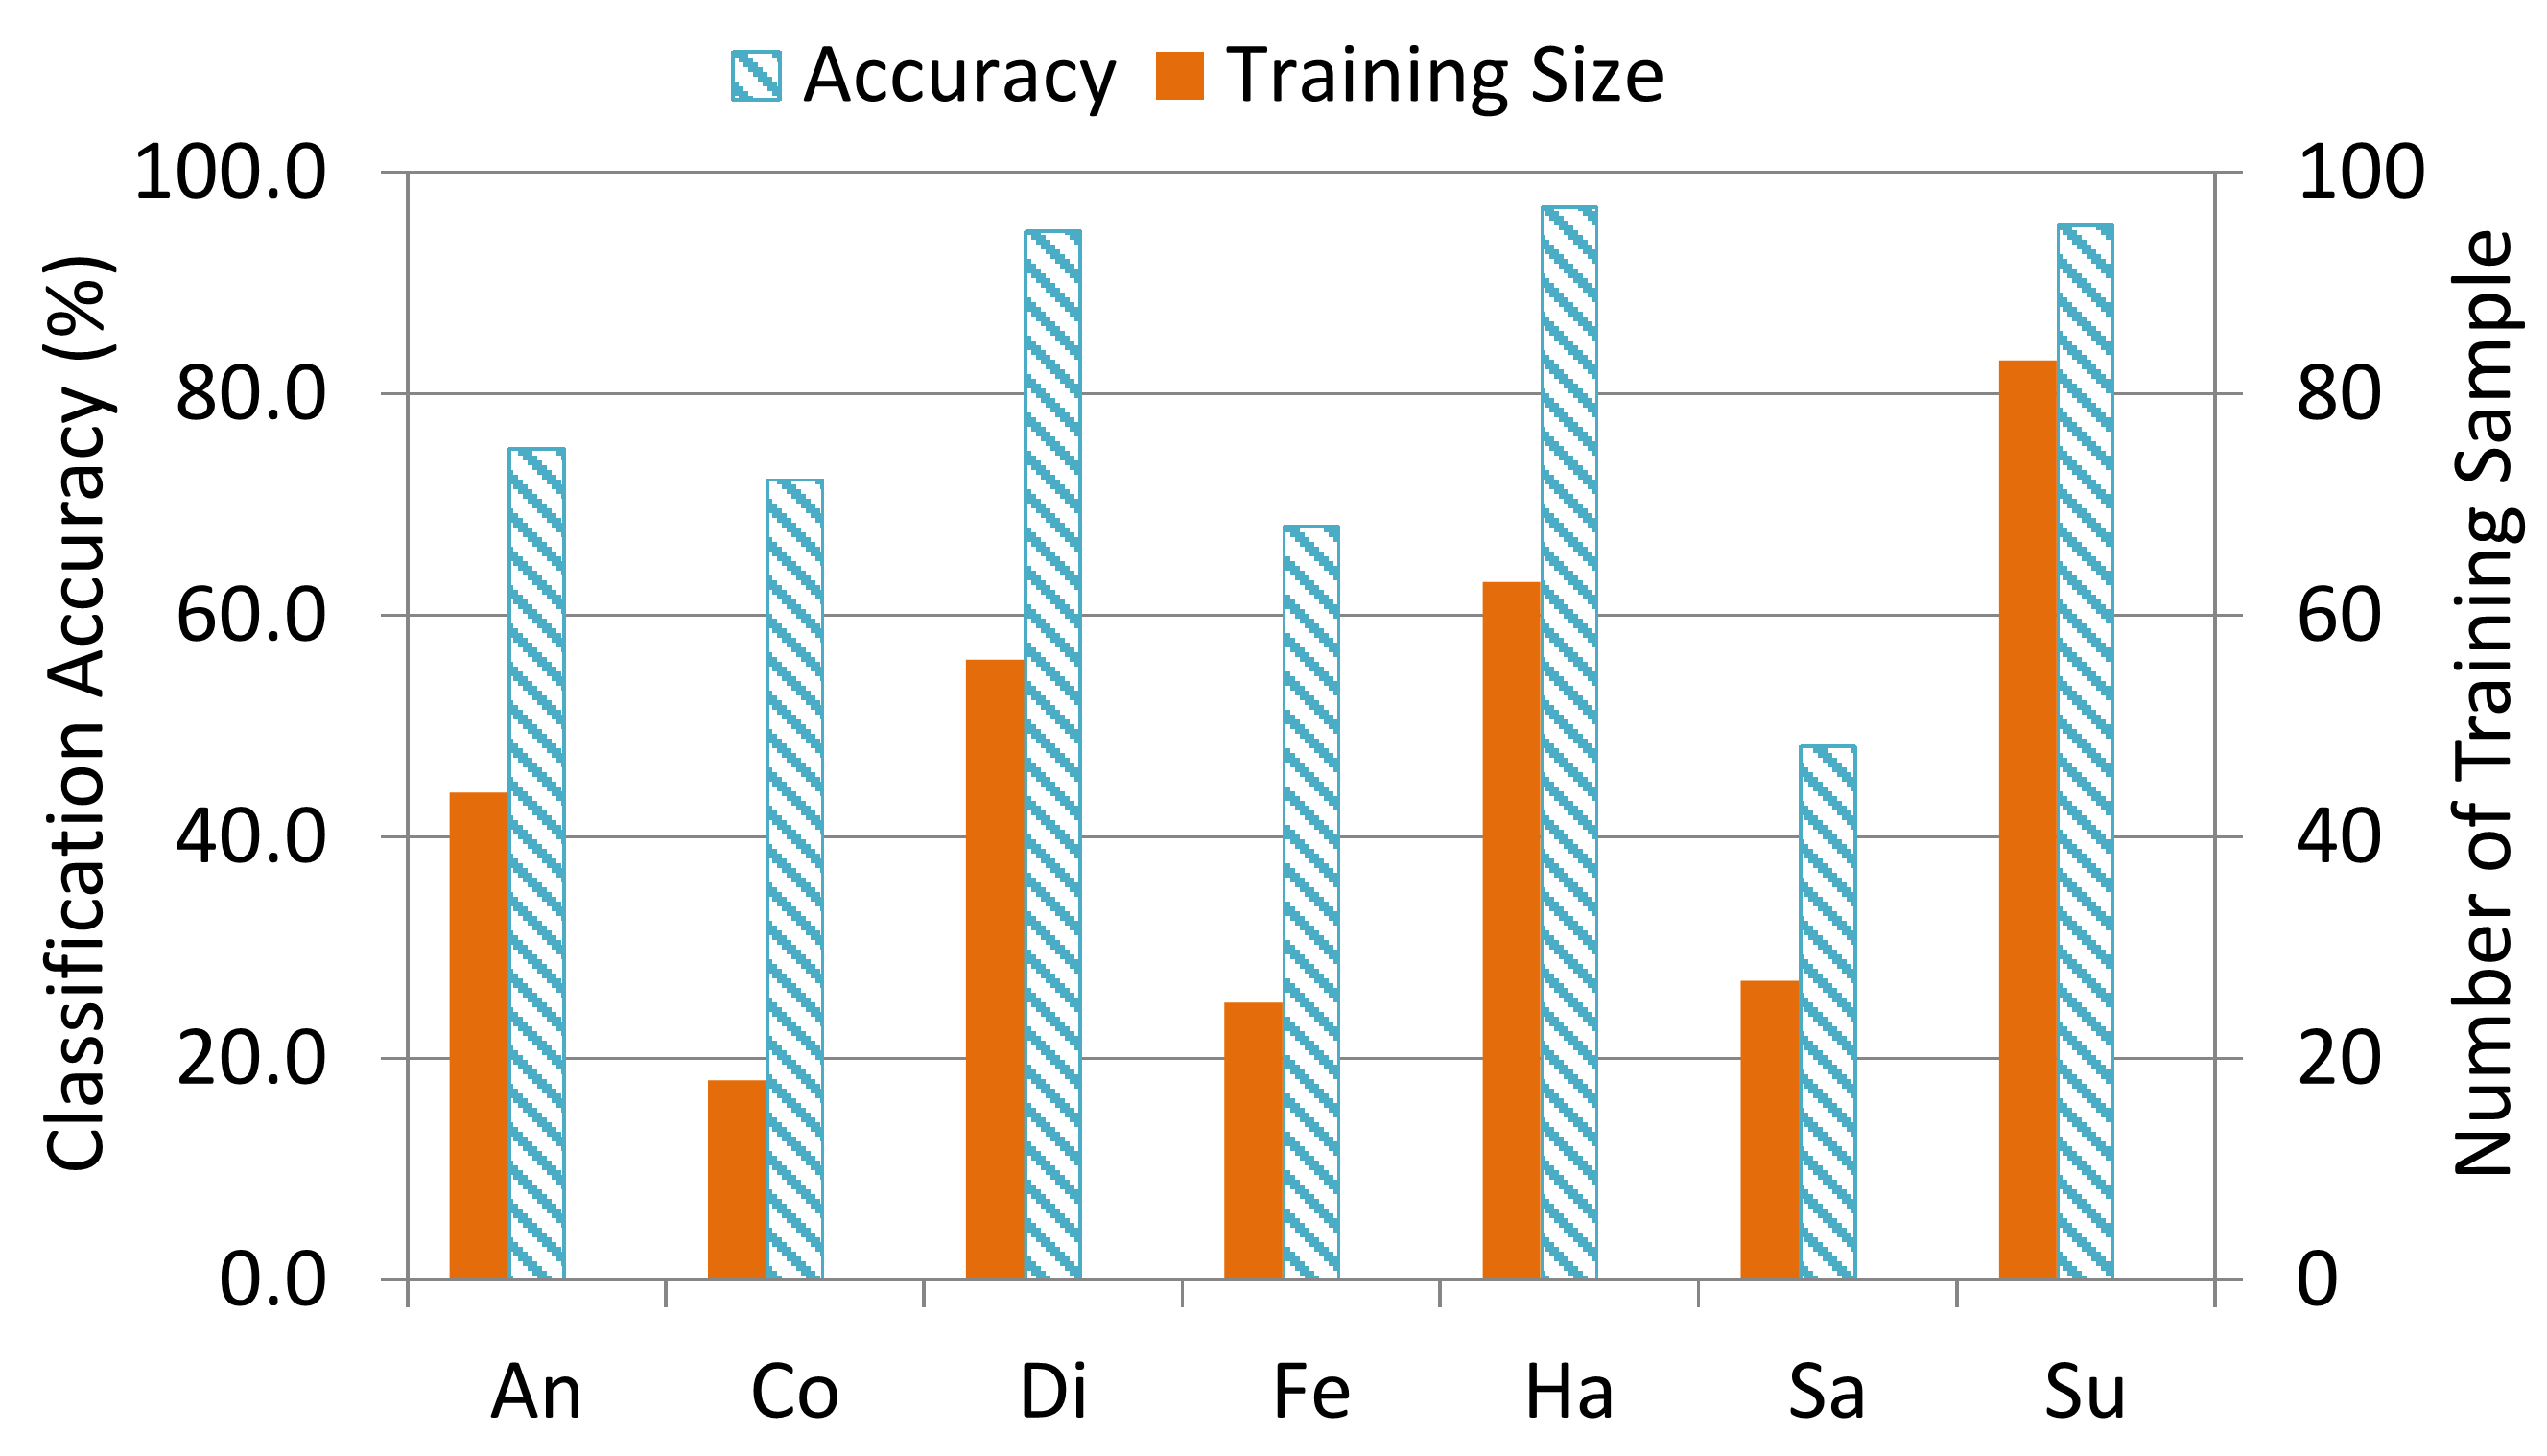
\includegraphics[width=.8\columnwidth]{pics/fig_ck_size.png}
	\caption{Relationship between the classification accuracy and the training size for each expression category. The accuracy is generally higher for categories with more training data.}
	\label{fig:fig_ck_size}
\end{figure}



\section{Conclusions\label{sec:conclude}}
We have proposed a low-rank sparse recovery framework to effectively extract dynamic muscle motion for unconstrained person-independent facial expression recognition in videos. Our approach decomposes a facial expression sequence into two representations, namely the Low-Rank Expression (LRE) and the Sparse Expression Residual (SER). The LRE recovers the underlying expression appearance shared in the entire expression sequence, while the SER captures the local muscle motion. The LRE and SER complement each other for a better expression recognition performance. Extensive experimental results have demonstrated the effectiveness of the proposed method and superior performance has been observed as compared to the state-of-the-art techniques. In addition, our approach has the potential of improvement given more samples from a larger training population. 

% Can use something like this to put references on a page
% by themselves when using endfloat and the captionsoff option.
\ifCLASSOPTIONcaptionsoff
  \newpage
\fi


\bibliographystyle{IEEEtran}
\bibliography{expression}

%\begin{IEEEbiography}[{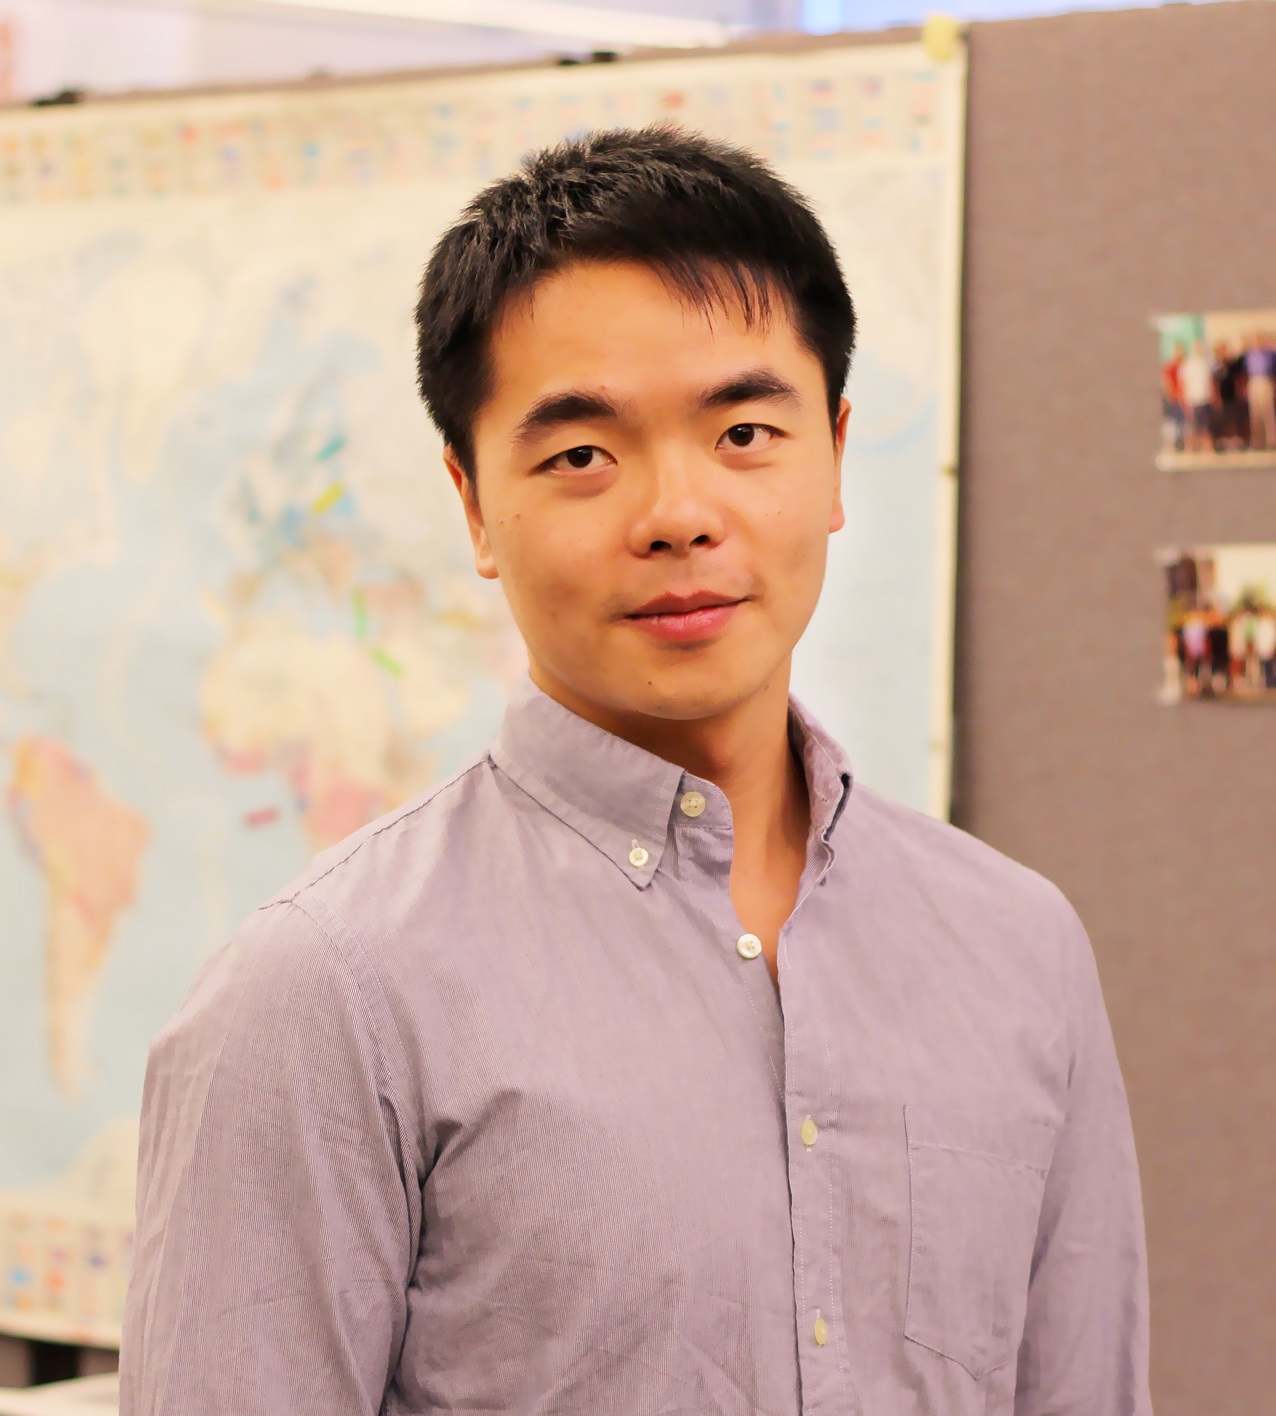
\includegraphics[width=1in,height=1.25in,clip,keepaspectratio]{photo/songfan.jpg}}]{Songfan Yang}
%(S'10-M'14) received the B.S. degree in Electrical Engineering from Sichuan University, Chengdu, China, in 2009 and the M.S. and Ph.D. degree in Electrical Engineering from University of California, Riverside. He is currently an Associate Professor of College of Electronics and Information Engineering at Sichuan University. His research interests include computer vision, pattern recognition, and affective computing. He holds the Best Entry Award of the FG 2011 Facial Expression Recognition and Analysis emotion challenge (FERA) competition.
%\end{IEEEbiography}
%
%\begin{IEEEbiography}[{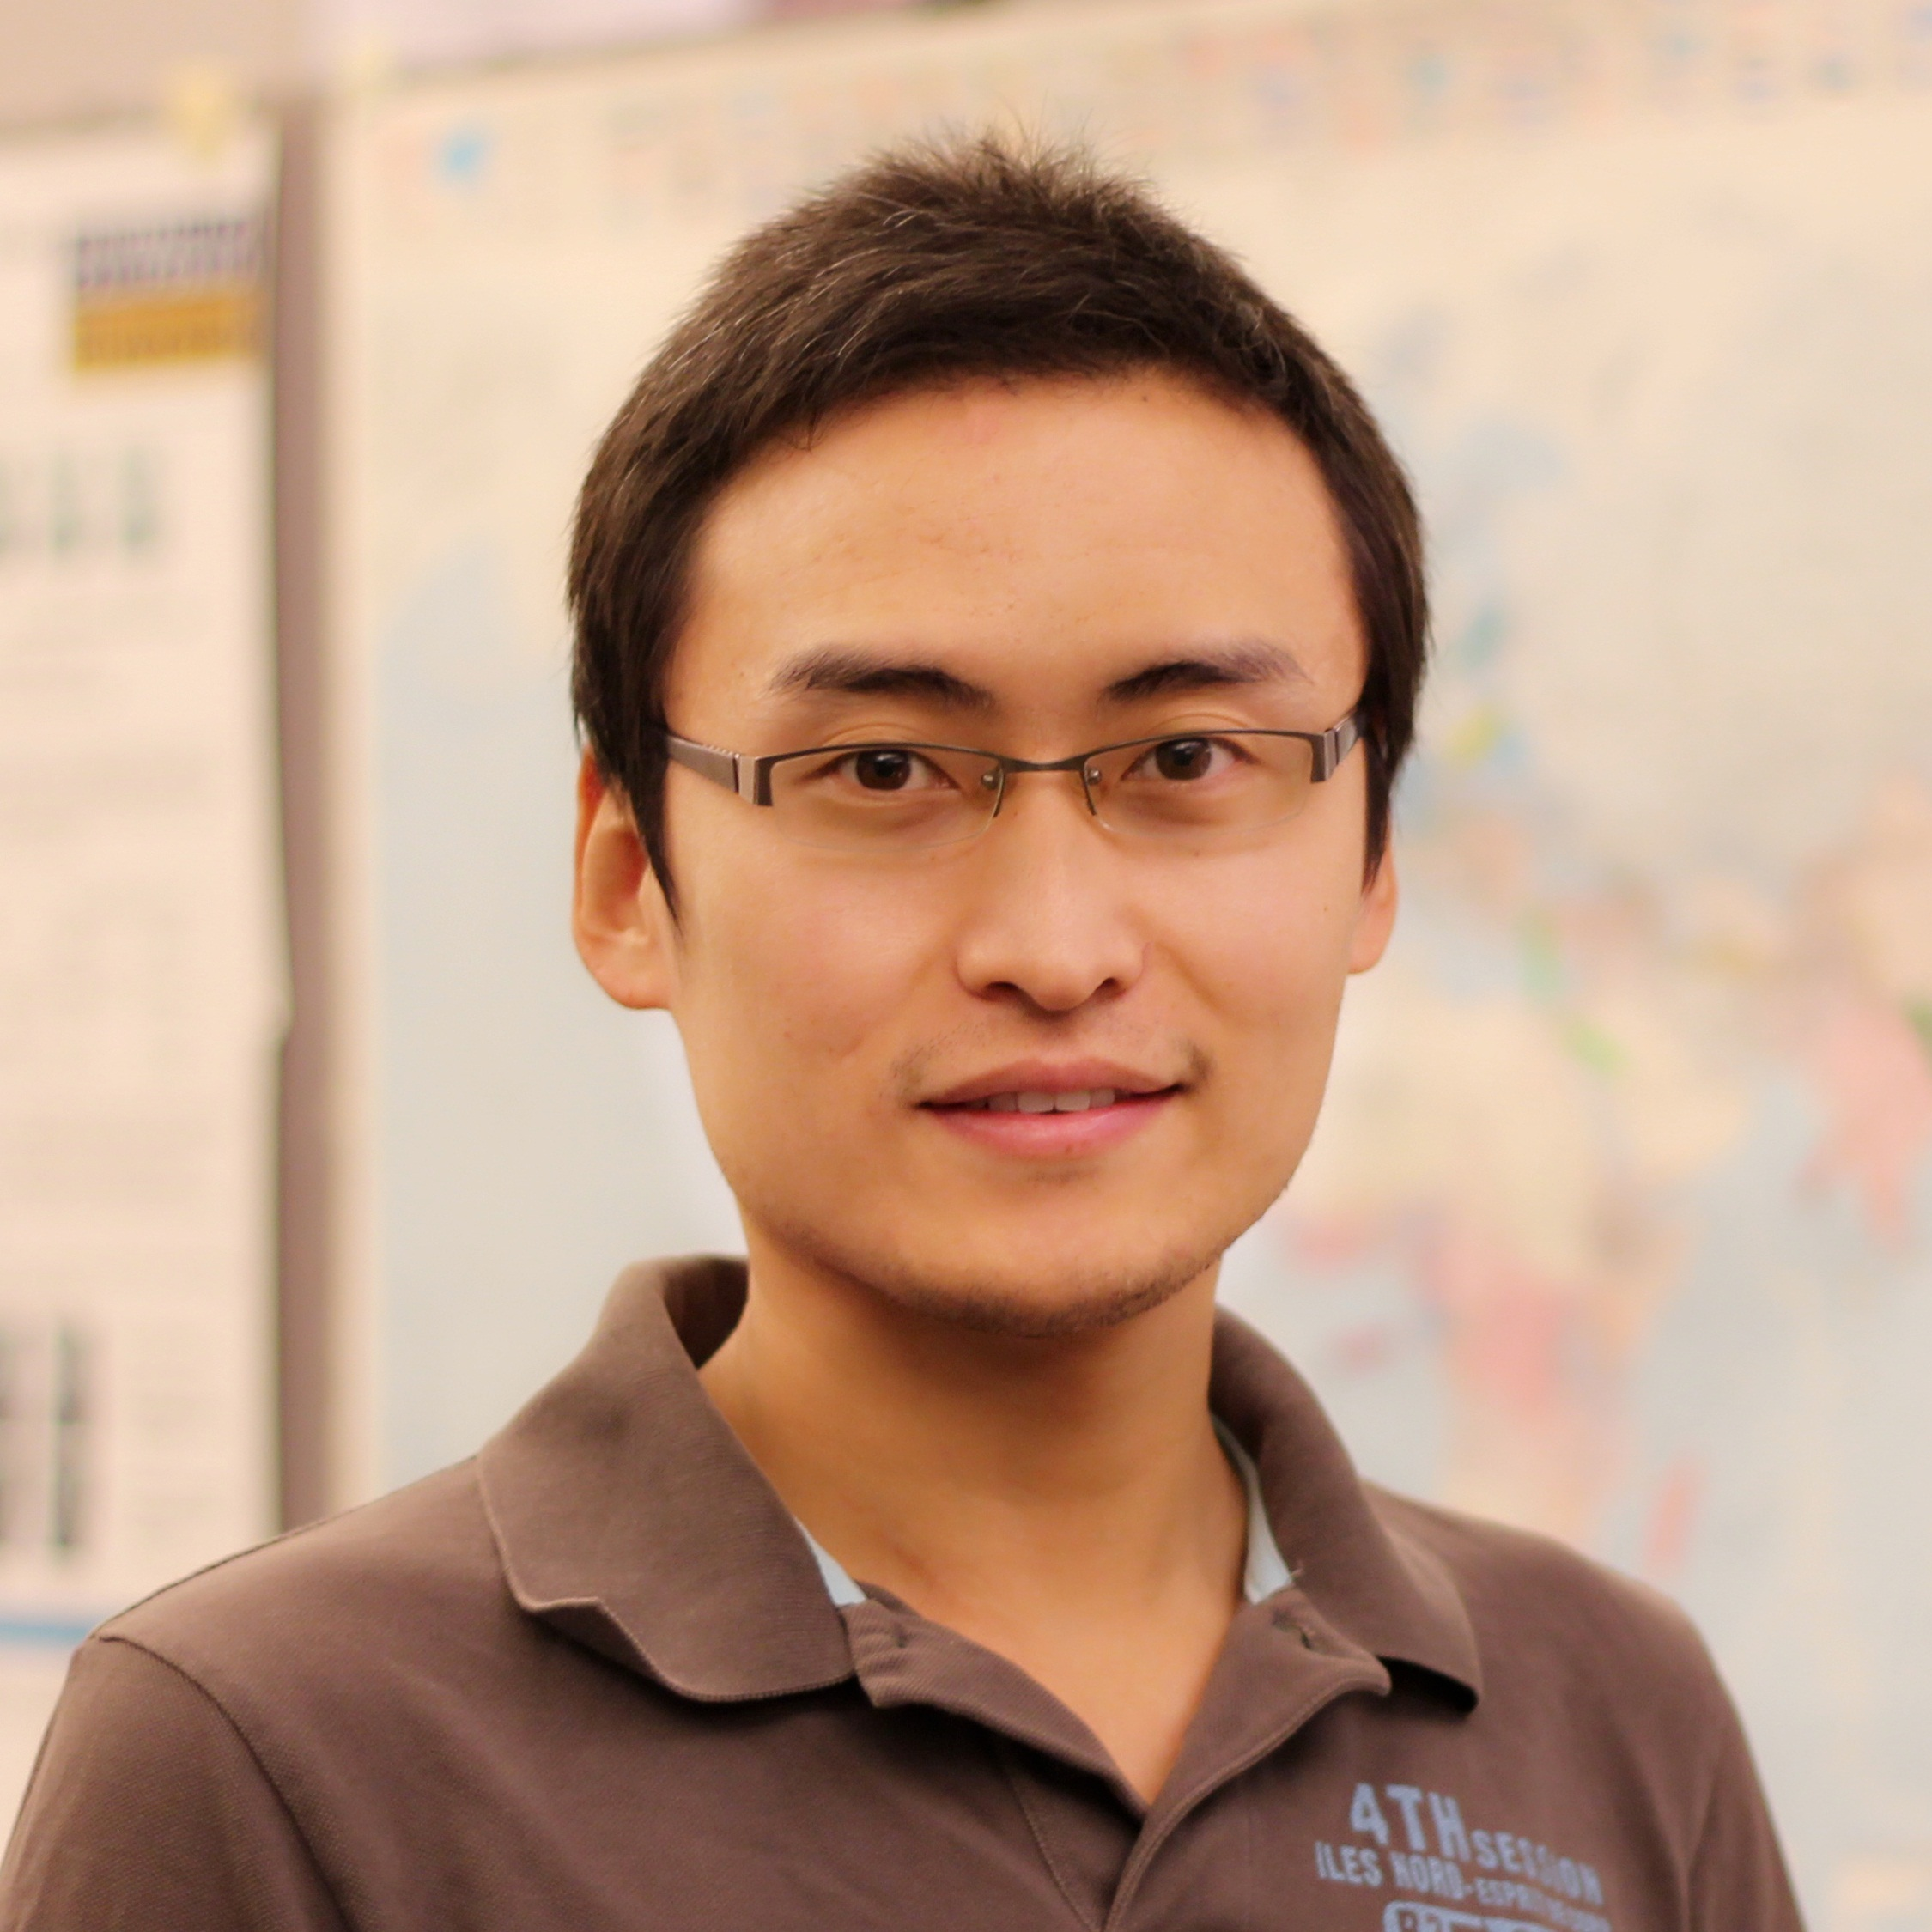
\includegraphics[width=1in,height=1.25in,clip,keepaspectratio]{photo/Lean.jpg}}]{Le An} received the B.Eng. degree in telecommunications engineering from Zhejiang University in China in 2006, the MSc degree in electrical engineering from Eindhoven University of Technology in Netherlands in 2008, and the PhD degree in electrical engineering from University of California, Riverside in USA in 2014. He is currently a postdoctoral research associate at University of North Carolina at Chapel Hill, USA.  
%His research interests include image processing, computer vision, pattern recognition, and machine learning. He received the best paper award from the 2013 IEEE International Conference on Advanced Video and Signal-Based Surveillance (AVSS).
%\end{IEEEbiography}
%
%\begin{IEEEbiography}[{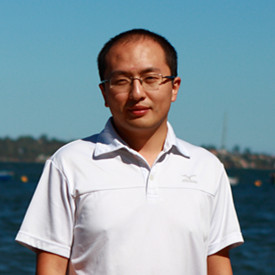
\includegraphics[width=1in,height=1.25in,clip,keepaspectratio]{photo/yinjie.jpg}}]{Yinjie Lei} received his MS degree from Sichuan University (SCU), China, in the area of image processing, and the Ph.D. degree in Computer Vision from University of Western Australia (UWA), Australia. He is currently an Assistant Professor at Sichuan University, Chengdu, China. He authored more than 10 peer reviewed journal and conference publications. He served as a reviewer for several international journals and several conferences. His research interests include image and text understanding, 3D face processing and recognition, 3D modeling, machine learning and statistical pattern recognition.
%\end{IEEEbiography}
%
%
%
%\begin{IEEEbiography}[{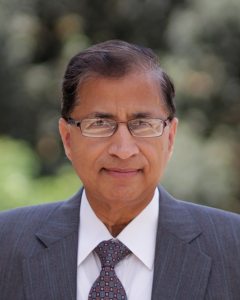
\includegraphics[width=1in,height=1.25in,clip,keepaspectratio]{photo/bhanu}}]{Bir Bhanu}
%(S'72-M'82-SM'87-F'95) received the S.M. and E.E. degrees in Electrical Engineering and Computer Science from the Massachusetts Institute of Technology, Cambridge, MA, the Ph.D. degree in Electrical Engineering, from the Image Processing Institute at University of Southern California and the M.B.A. degree from the University of California, Irvine. He is the Distinguished Professor of Electrical Engineering and Cooperative Professor of Computer Science and Engineering, Mechanical Engineering and Bioengineering, and the Director of the Center for Research in Intelligent Systems (CRIS) and the Visualization and Intelligent Systems Laboratory (VISLab) at the University of California, Riverside (UCR). In addition, he serves as the director of NSF IGERT on Video Bioinformatics at UCR. Dr. Bhanu has been the Principal Investigator of various programs for NSF, DARPA, NASA, AFOSR, ONR, ARO, and other agencies and industries in the areas of video networks, video understanding, video bioinformatics, learning and vision, image understanding, pattern recognition, target recognition, biometrics, autonomous navigation, image databases, and machine-vision applications. He has published seven coauthored and three edited books. He is the holder of 18 (5 pending) patents. He has published more than 450 reviewed technical publications, including over 120 journal papers and 45 book chapters. His current research interests are Computer Vision, Pattern Recognition and Data Mining, Machine Learning, Artificial Intelligence, Image Processing, Image and Video Database, Graphics and Visualization, Robotics, Human-Computer Interactions, Biological, Medical, Military and Intelligence applications. He is Fellow of IEEE, AAAS, IAPR, and SPIE.
%\end{IEEEbiography}

% that's all folks
\end{document}


